\documentclass{article}

% Language setting
% Replace `english' with e.g. `spanish' to change the document language
\usepackage[english]{babel}

% Set page size and margins
% Replace `letterpaper' with `a4paper' for UK/EU standard size
\usepackage[a4paper,top=2cm,bottom=2cm,left=3cm,right=3cm,marginparwidth=1.75cm]{geometry}

% Useful packages
\usepackage{amsmath}
\DeclareMathOperator{\sinc}{sinc}
\DeclareMathOperator*{\argmax}{arg\,max}
\DeclareMathOperator*{\argmin}{arg\,min}
\usepackage{cancel}
\usepackage{amssymb}
\usepackage{float}
\usepackage{graphicx}
\usepackage[colorlinks=true, allcolors=blue]{hyperref}

\usepackage{tikz}
\usetikzlibrary{arrows,decorations.pathmorphing,backgrounds,fit,positioning,shapes.symbols,chains,shapes.geometric,shapes.arrows,calc}

\usepackage{listings}
\usepackage{xcolor}
\usepackage{enumitem}
\usepackage{physics}
\setlist[itemize]{nosep} 

\definecolor{codegreen}{rgb}{0,0.6,0}
\definecolor{codegray}{rgb}{0.5,0.5,0.5}
\definecolor{codepurple}{rgb}{0.58,0,0.82}
\definecolor{backcolour}{rgb}{0.95,0.95,0.92}

\lstdefinestyle{mystyle}{
  backgroundcolor=\color{backcolour},   
  commentstyle=\color{codegreen},
  keywordstyle=\color{magenta},
  numberstyle=\tiny\color{codegray},
  stringstyle=\color{codepurple},
  basicstyle=\ttfamily\footnotesize,
  breakatwhitespace=false,         
  breaklines=true,                 
  captionpos=b,                    
  keepspaces=true,                 
  numbers=left,                    
  numbersep=5pt,                  
  showspaces=false,                
  showstringspaces=false,
  showtabs=false,                  
  tabsize=2
}

\lstset{style=mystyle}

\title{Computer Vision}
\author{Matteo Galiazzo}

\begin{document}

\maketitle

\tableofcontents

% lecture 1

\section{Introduction}

The difference between computer vision and image processing is the fact that computer vision is the process of extracting information from images, while image processing aims at improving the quality of images.
Quite often image processing helps computer vision.
The informations we want to extract from the images could be counting, object orientation, object classification, measurements...
Computer vision is challenging since we lose depth from the images (3D information becomes 2D), scale and illumination varies, and there's object occlusion (object hiding other objects).

Computer vision started with hand-crafted decision rules that only required few images as example, and evolved to machine learning where the algorithm learns a decision rule, but the training requires hundreds to thousands of images.
The big paradigm shift happened with deep learning (e2e learning) which learned both the image representation and the decision rules, but required thousands to millions of words.
Deep learning has been enabled by better networks, better hardware and more data.


\section{Fundamentals of Image Processing and Computer Vision}
% lecture 2

\subsection{Images}

An imaging device gathers the light reflected by 3D objects to create a 2D representation of the scene.

\subsubsection{Pinhole camera model}
The "pinhole camera" is the simplest camera model we can define.
Light goes through the very small pinhole (to not have saturation) and hits the image plane.
Geometrically, the image is achieved by drawing straight rays from scene points through the hold up to the image plane.

This simple geometrical model turns out to be a good approximation of the geometry of image formation.
However, useful images can hardly be captured by means of a pinhole camera.

The \textbf{geometric model of image formation} in a pinhole camera is known as \textbf{perspective projection}.

\begin{figure}[htbp]
  \centering
  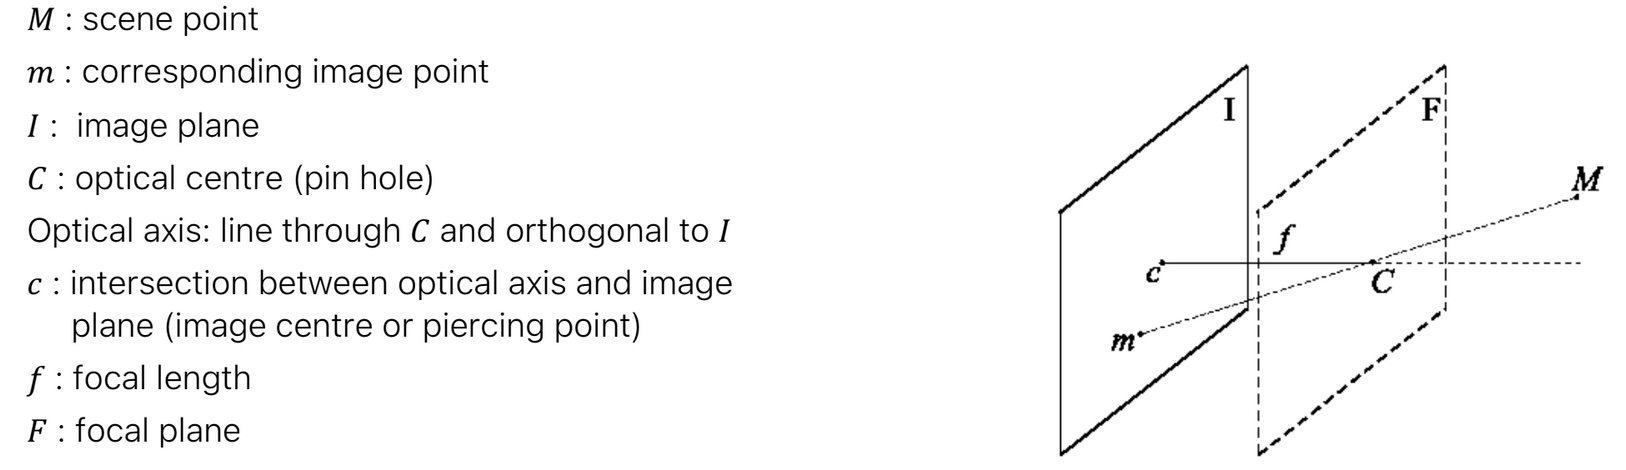
\includegraphics[width=0.9\linewidth]{./img/perspective_projection.jpg}
  \caption{perspective projection}
\end{figure}

Which, by writing the poitns as vectors and the plane's coordinates, becomes the geometric model in the image \ref{fig:perspective_projection_axis}

\begin{figure}[htbp]
  \centering
  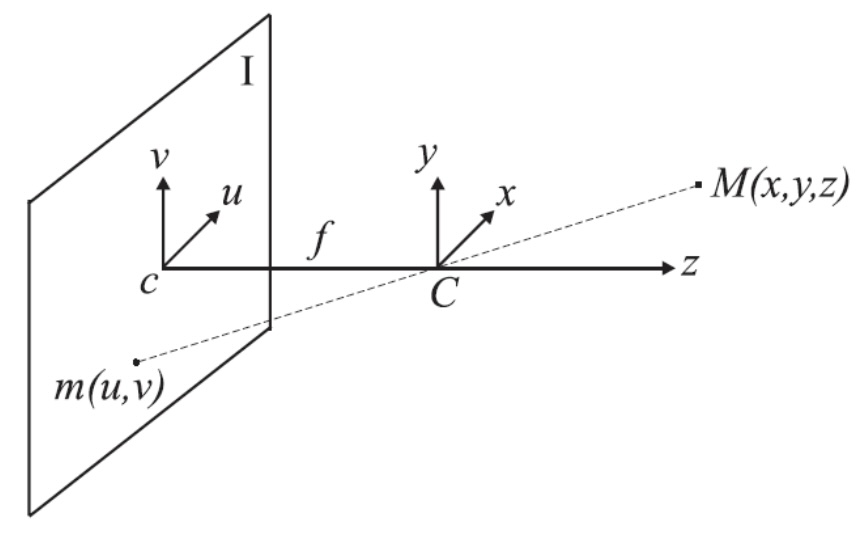
\includegraphics[width=0.45\linewidth]{./img/perspective_projection_axis.jpg}
  \caption{geometric model of image formation}
  \label{fig:perspective_projection_axis}
\end{figure}

Given the reference frame in the image \ref{fig:perspective_projection_axis} 
\begin{itemize}
  \item $u$ is the horizontal axis in the image plane.
  \item $v$ is the vertical axis in the image plane.
  \item $X$ and $Y$ are the respective axis in the 3D reference system. It's called the \textbf{camera reference system} because it is "attached" to the camera.
\end{itemize}

\textbf{For the perspective model these axis must be parallel}

The equations to map scene points into their corresponding image points are defined as:

$$\frac{u}{x} = -\frac{f}{z} \rightarrow u = -x\frac{f}{z} \quad\quad\quad \frac{v}{y} = - \frac{f}{z} \rightarrow v = -y\frac{f}{z}$$

The minus sign means the axis gets inverted (as we can see in the visualization, and it's what happens in the brain).
We can get rid of the sign, since the image plane can be though of as lying in front rather than behind the optical centre.

Image coordinates are a scaled version of scene coordinates (function of depth).
When $z$ increases, since it's at the denominator in both the equations, the terms gets smaller (object gets smaller in the image).
When $f$ increases, since it's at the numerator in both the equations the term gets bigger (object gets bigger in the image)

As we previously said, the image formation process deals with mapping a 3D space onto a 2D space, and so to the loss of depth information.
A given scene point is mapped into an image point, but an image point is mapped onto a 3D line.
For an image point we can only state that its corresponding scene point lays on a line, but cannot disambiguate a specific 3D point along the line.

\subsubsection{Stereo images}

We use multiple images to create stereo vision.
Given correspondences, 3D information can be recovered easily by triangulation.
We can use two cameras, or two cameras and an infrared sensor to project guides to align the images.

For standard stereo geometry there are some assumptions we have to make:
\begin{itemize}
  \item The cameras have parallel $(x,y,z)$ axes.
  \item The image planes of both cameras are coplanar and aligned.
  \item Both cameras have identical focal lengths.
\end{itemize}
\vspace{1em}
Based on this, the transformation between the two reference frames is just a translation, usually horizontal.
For stereo vision is also really important to \textbf{sense two images at the same moment}.

The cameras are displaced at a given quantity $b$ called baseline.
The \textbf{disparity} is the difference between the horizontal coordinates in the left and right images.

\begin{figure}[htbp]
  \centering
  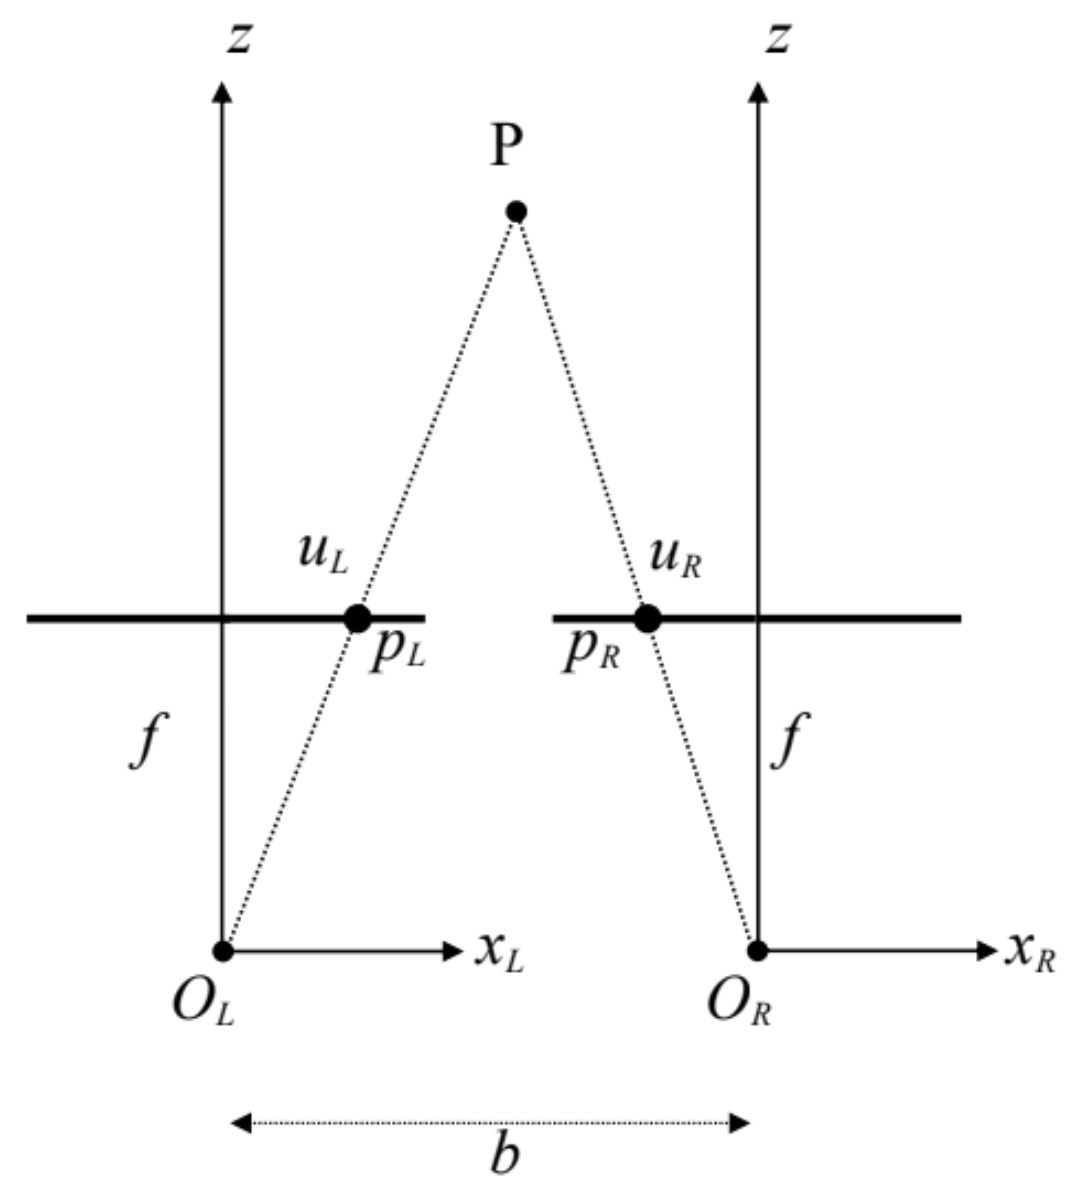
\includegraphics[width=0.45\linewidth]{./img/standard_stereo_geometry.jpg}
  \caption{standard stereo geometry}
  \label{fig:standard_stereo_geometry}
\end{figure}

% The fundamental relationship in stereo vision is $z = b \cdot \frac{f}{d}$.
% It's used to calculate the depth of a point in a scene from a pair of stereo images.

In standard stereo geometry since we are given just two 2D images there is no info about the correspondence between two points in the two images.
We can recall that the camera have parallel axes, and so we know that we can search for the correspondence along the horizontal lines.
This task is called stereo matching.

\subsubsection{Stereo correspondence}
In stereo correspondence, given a point in one image, we have to find it in the other image which is the projection of the same 3D point.
Such image points are called corresponding points.
\textbf{Points farther away have a smaller disparity, while close points have a larger display}.

\begin{figure}[htbp]
  \centering
  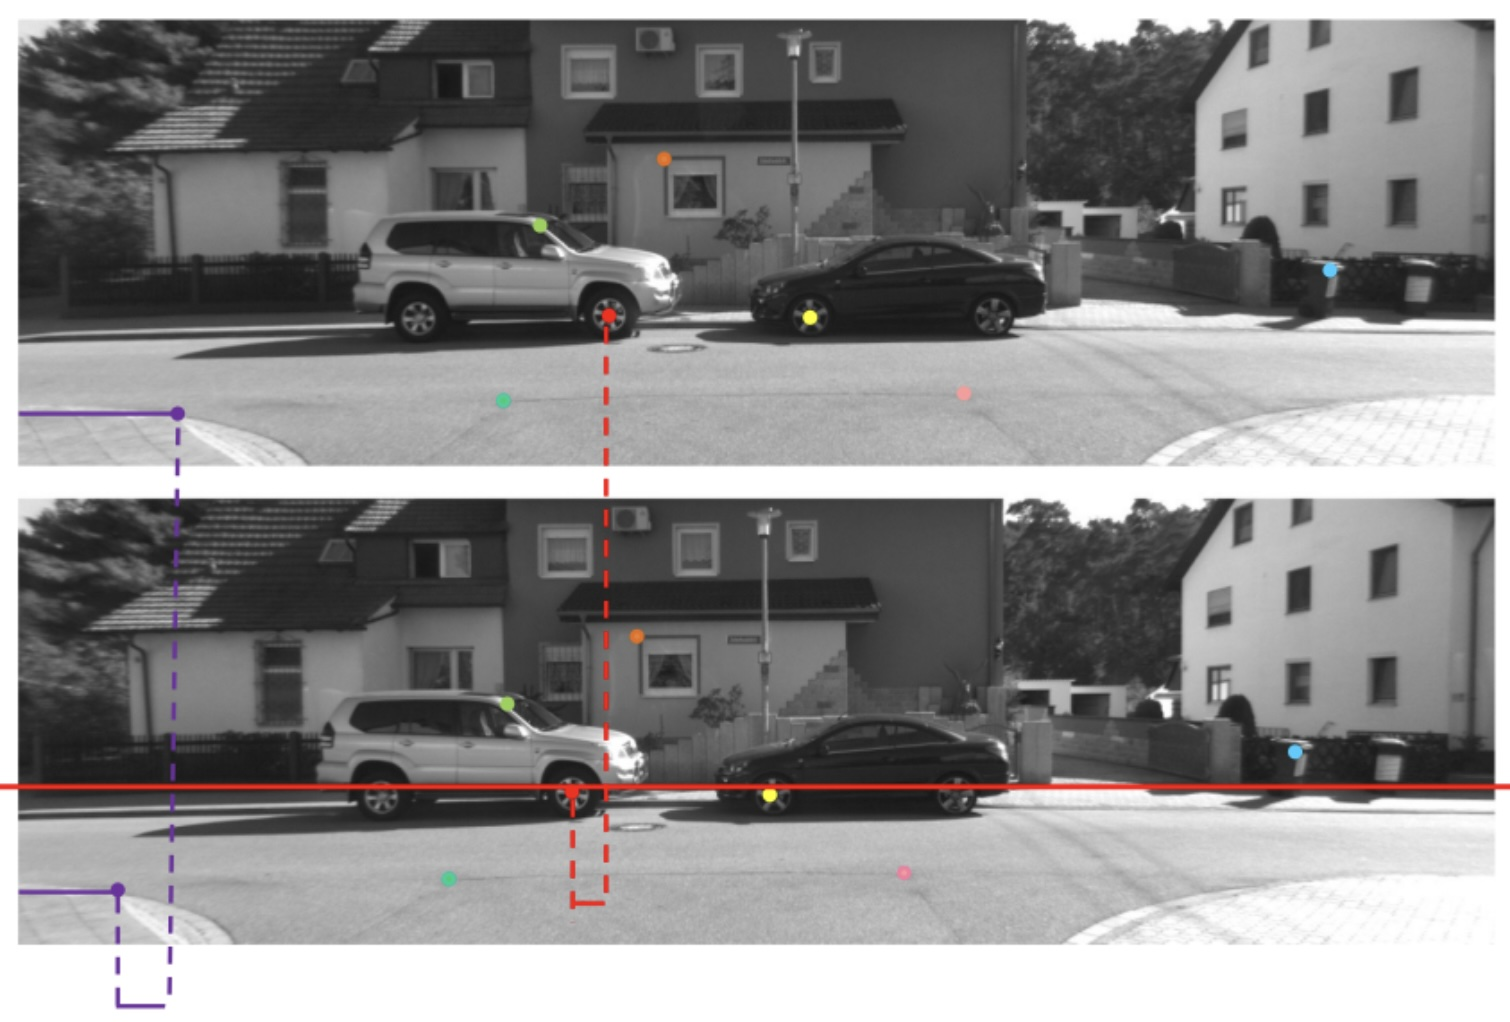
\includegraphics[width=0.65\linewidth]{./img/stereo_correspondence.jpg}
  \caption{Corresponding points look similar in the two images}
  \label{fig:stereo_correspondence}
\end{figure}

The image of a 3D line segment of length $L$ lying in a plane parallel to the image plane at distance $z$ from the optical centre will exhibit a length given by:
$$l = L \frac{f}{z}$$
This relationship is more complicated for an arbitrarily oriented 3D segment, as its position and orientation need to be accounted for as well.
For a \textbf{given position and orientation, length always shrinks alongside distance}.

Perspective projection maps 3D lines into image lines.
\textbf{Parallelism between 3D lines is not preserved} (except for lines parallel to the image plane).
This is the reason why if we look at a really long road into the distance we have the perception that the road becomes thinner, and the lines of the road intersect in the distance.
The images of parallel 3D lines intersect at a point, called \textbf{vanishing point}, which isn't necessarily within the image.

If the lines are parallel to the image plane they meet at infinity.

\subsubsection{Epipolar geometry}

What if the two cameras are no longer aligned? Do we need to search through the whole image?
We can project the line related to point $P_L$ in the right plane and search across that line.
The issue is that this projection can be computed only if the transformation between the two cameras is known (the relative mapping between the two cameras).

\begin{figure}[htbp]
  \centering
  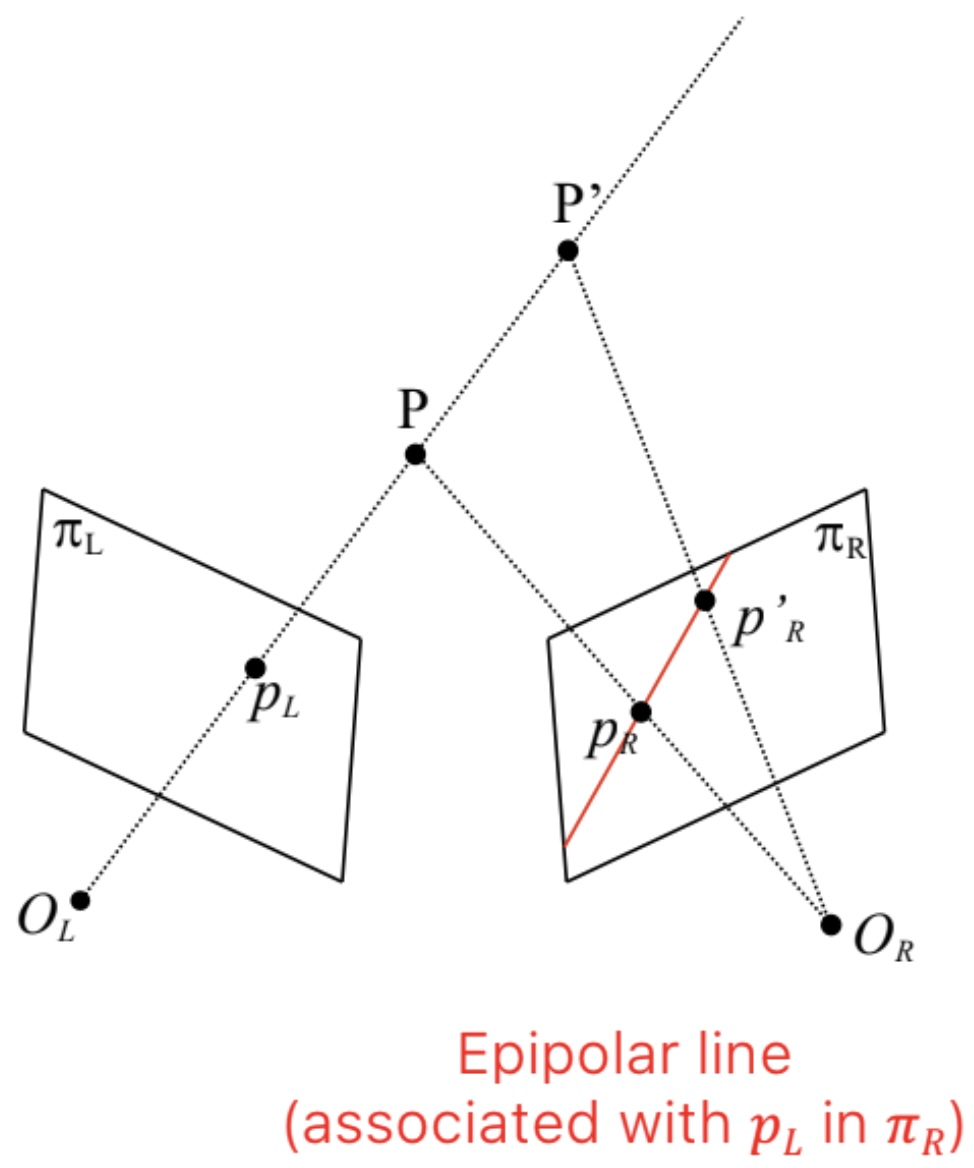
\includegraphics[width=0.45\linewidth]{./img/epipolar_line.jpg}
  \caption{Epipolar line}
  \label{fig:epipolar_line}
\end{figure}

It is almost impossible to build a stereo rig which is perfectly aligned horizontally.
Searching through oblique epipolar lines is awkward, and computationally is less efficient.
What people do in practice is to convert epipolar geometry to standard geometry with rectification/warping.
We warp the images as if they were acquired through a standard geometry, then we can compute and apply to both images a transformation known as rectification.

\subsubsection{Depth of Field (DOF)}

A scene point is on focus when all its light rays, gathered by the camera, hit the image plane at the same point.
In a pinhole device this happens to all scene points because of the very small size of the hole, so that the camera features an infinite Depth of Field (DOF).

The drawback is that such a small aperture allows gathering a very limited amount of light.
The image is really sharp, but has a really low light.
If a point is projected onto a circle instead of a point (bigger pinhole) the image is not sharp (not on focus).
If we cannot gather enough light through the aperture we have to integrate through time, by using a longer exposure time.

\subsubsection{Lenses}

Lenses concentrate light, so we use them to gather more light from a scene point and focus it on a single image point.
This enables much smaller exposure times.
This way Depth Of Field is no longer infinite, and only a limited range of points can be simultaneously on focus in a given image.

We will consider the approximate model known as thin lens equation, which is useful to graphically determine the position of a focused image point:
\begin{itemize}
  \item Rays parallel to the optical axis are deflected to pass through $F$.
  \item Rays through $C$ are undeflected.
\end{itemize}

\textbf{If the image is on focus}, the image formation process obeys to the perspective projection model:
\begin{itemize}
  \item The center of the lens is the optical center.
  \item The distance $v$ acts as the effective focal length of the projection.
\end{itemize}

\begin{figure}[htbp]
  \centering
  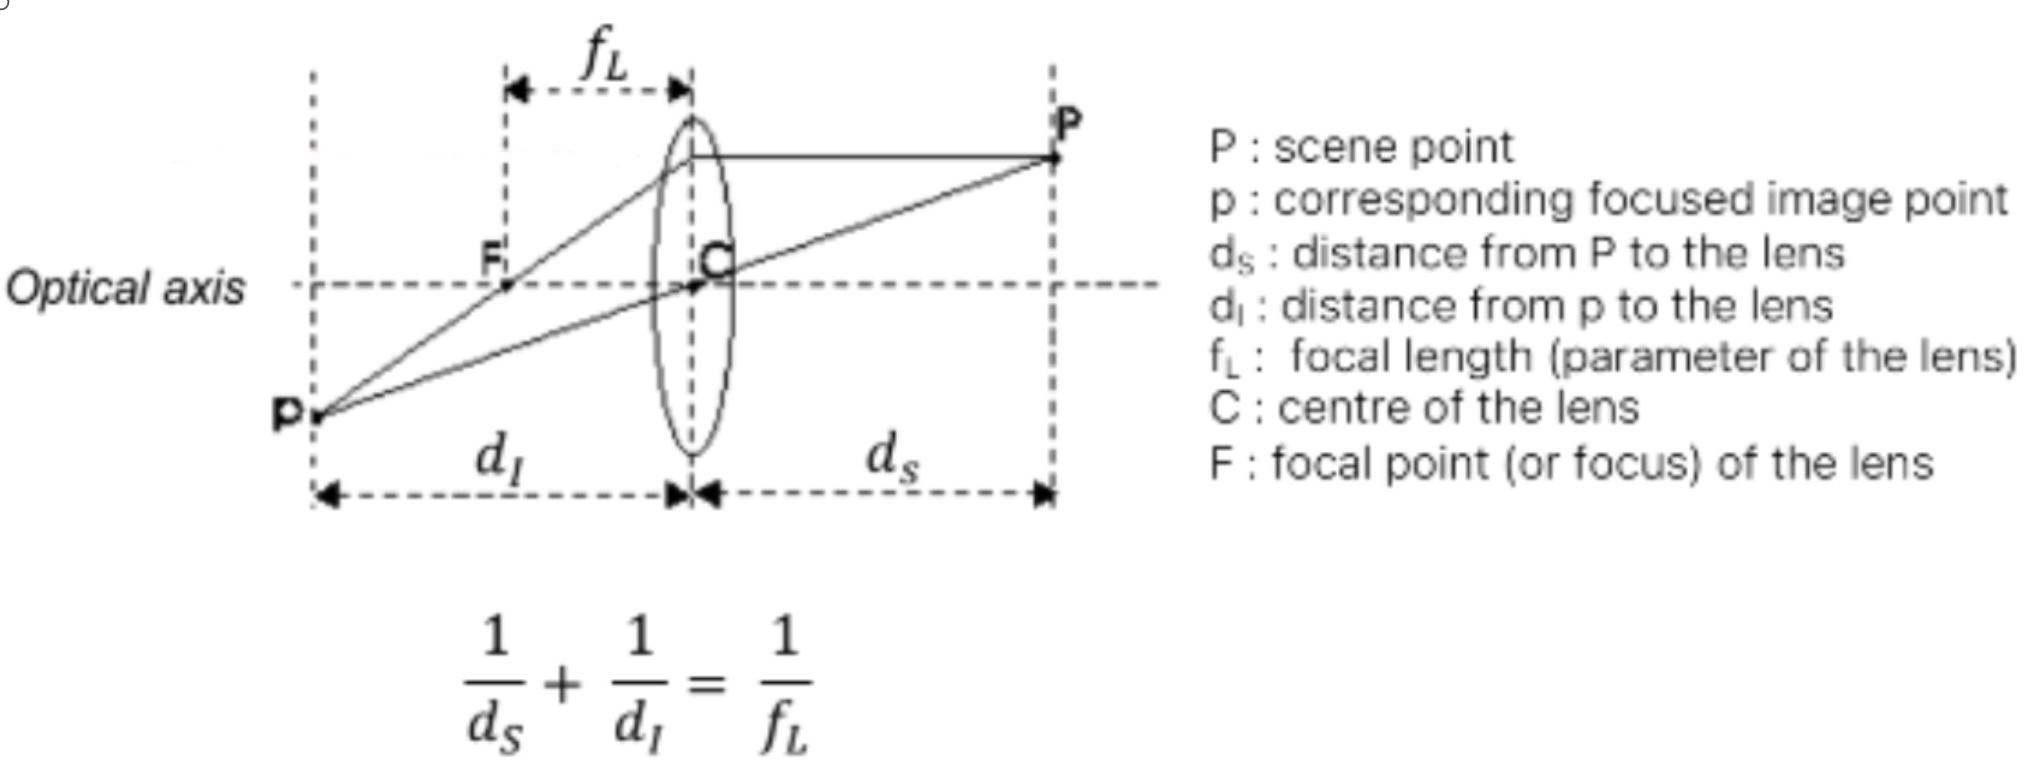
\includegraphics[width=0.7\linewidth]{./img/lens.jpg}
  \caption{Scheme of a lens}
  \label{fig:lens}
\end{figure}

Choosing the distance of the image plane determines the distance at which scene points appear on focus in the image.
Scene points in front and behind the focusing plane will result out-of-focus, thereby appearing in the image as \textbf{blur circles}, rather than points.

The advantage of lenses is to have a small exposure time for capturing moving objects but we pay in terms of Depth Of Field.

\begin{figure}[htbp]
  \centering
  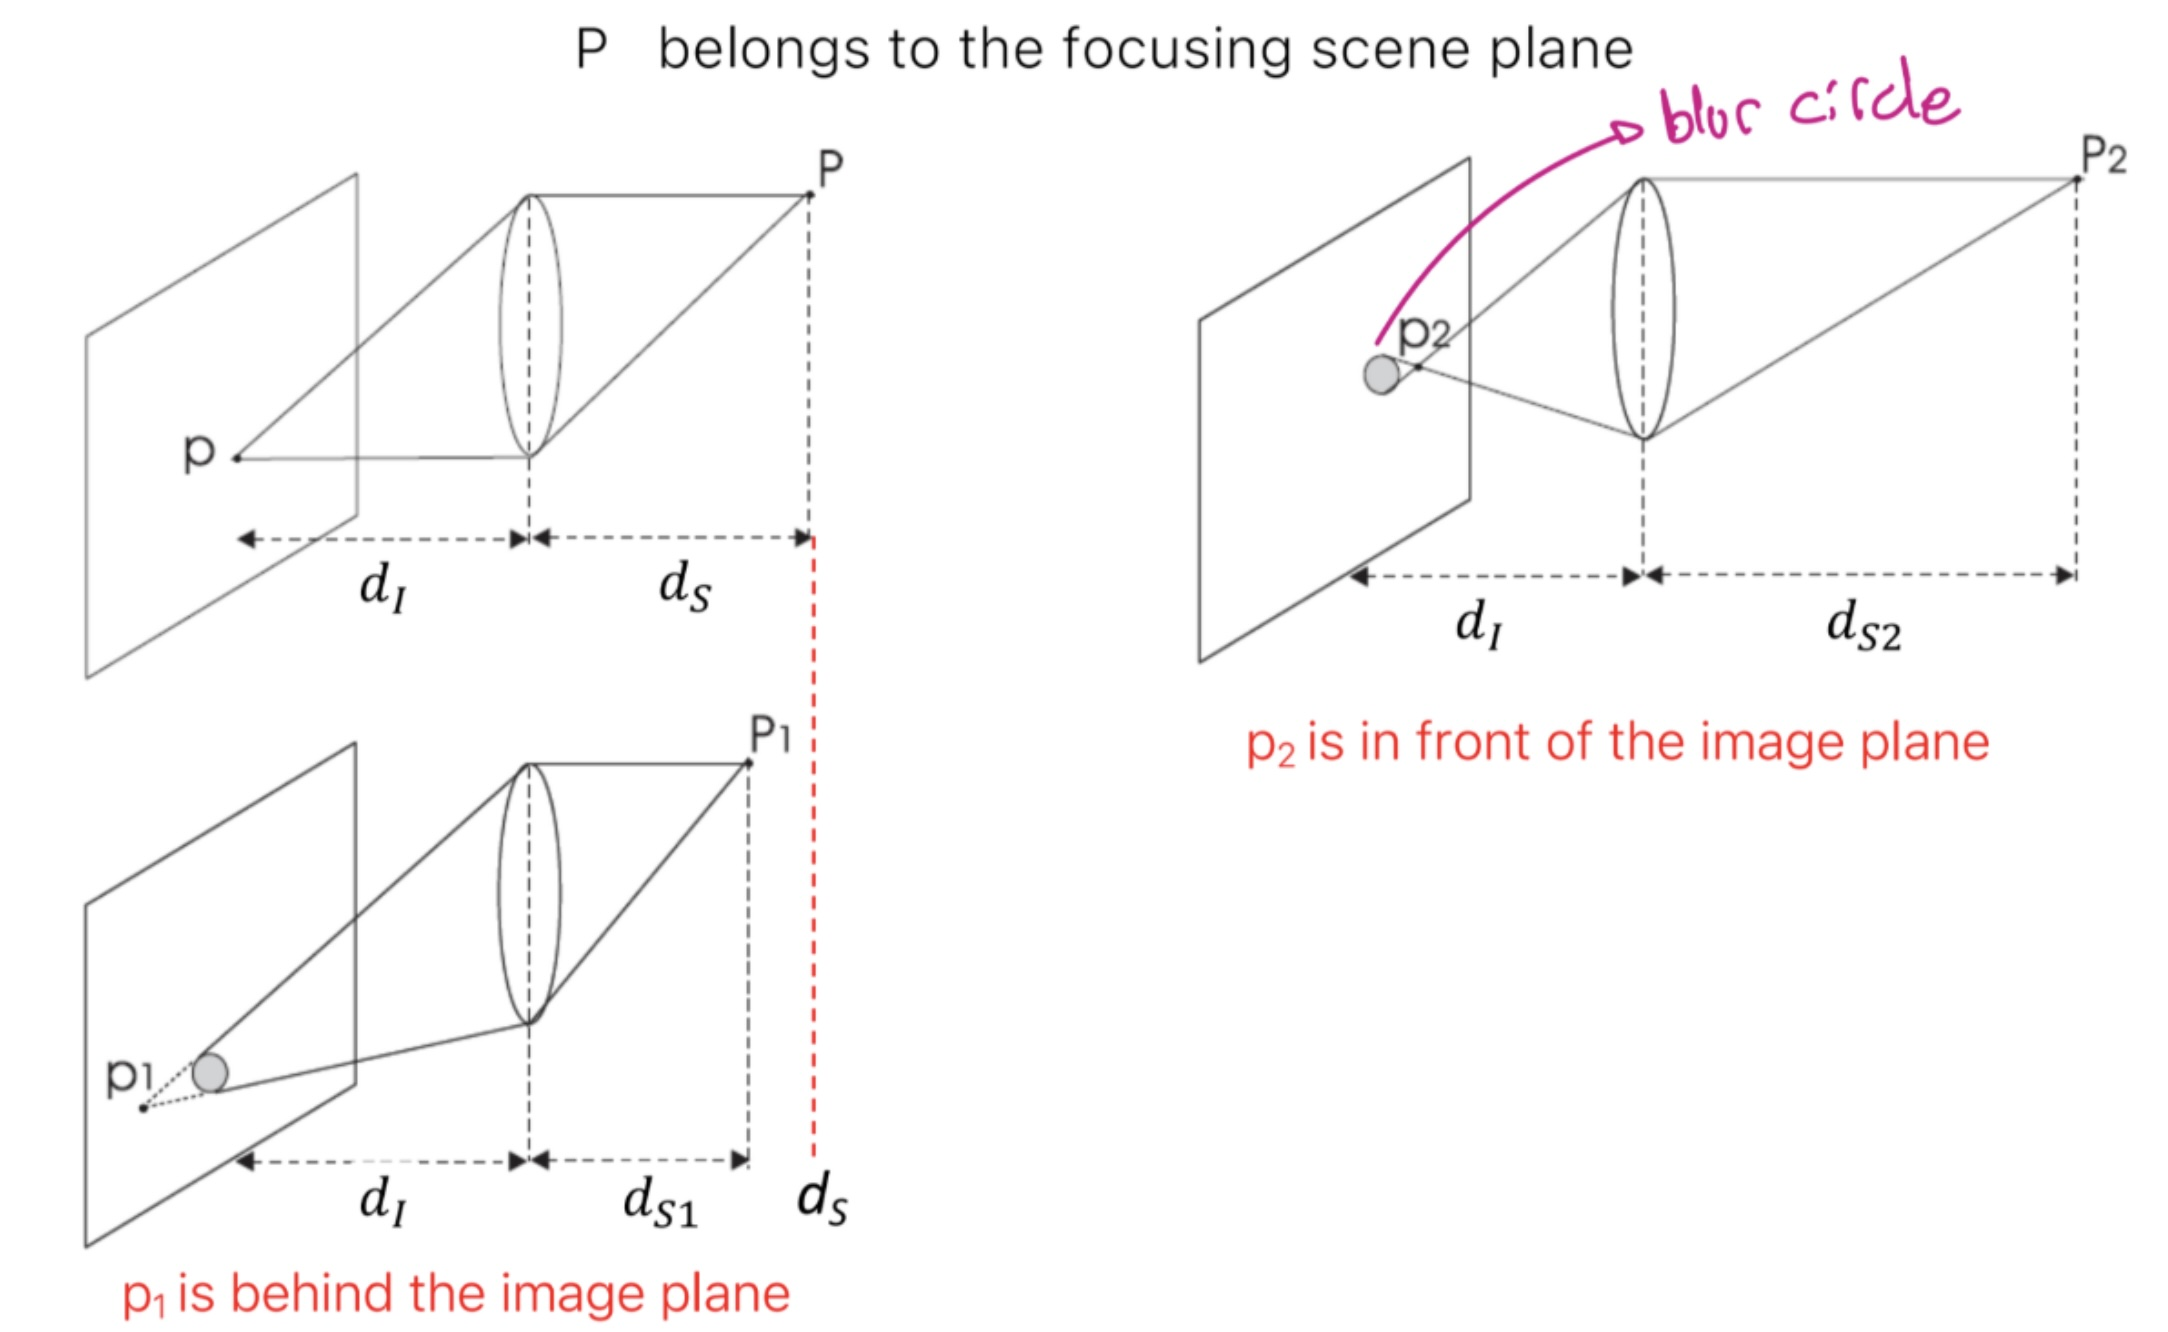
\includegraphics[width=0.8\linewidth]{./img/lens_focus.jpg}
  \caption{Lens focusing at various distances}
  \label{fig:lens_focus}
\end{figure}

As we can see in \ref{fig:tradeoffs} having a small aperture (pinhole camera model) results in everything being on focus, but we need lots of light, or the image will be dark, since few light can enter in the sensor.
We could also increase our exposure time to let more light in, but in that case we need the objects in our image to be still.
Having a bigger aperture results in more light coming in in a small time fraction, but the lens distortion causes the light to be focused only at certain distances, and creates blur cirlces in other zones, so we get a lower depth of field, as we can see in \ref{fig:lens_focus}.

\begin{figure}[htbp]
  \centering
  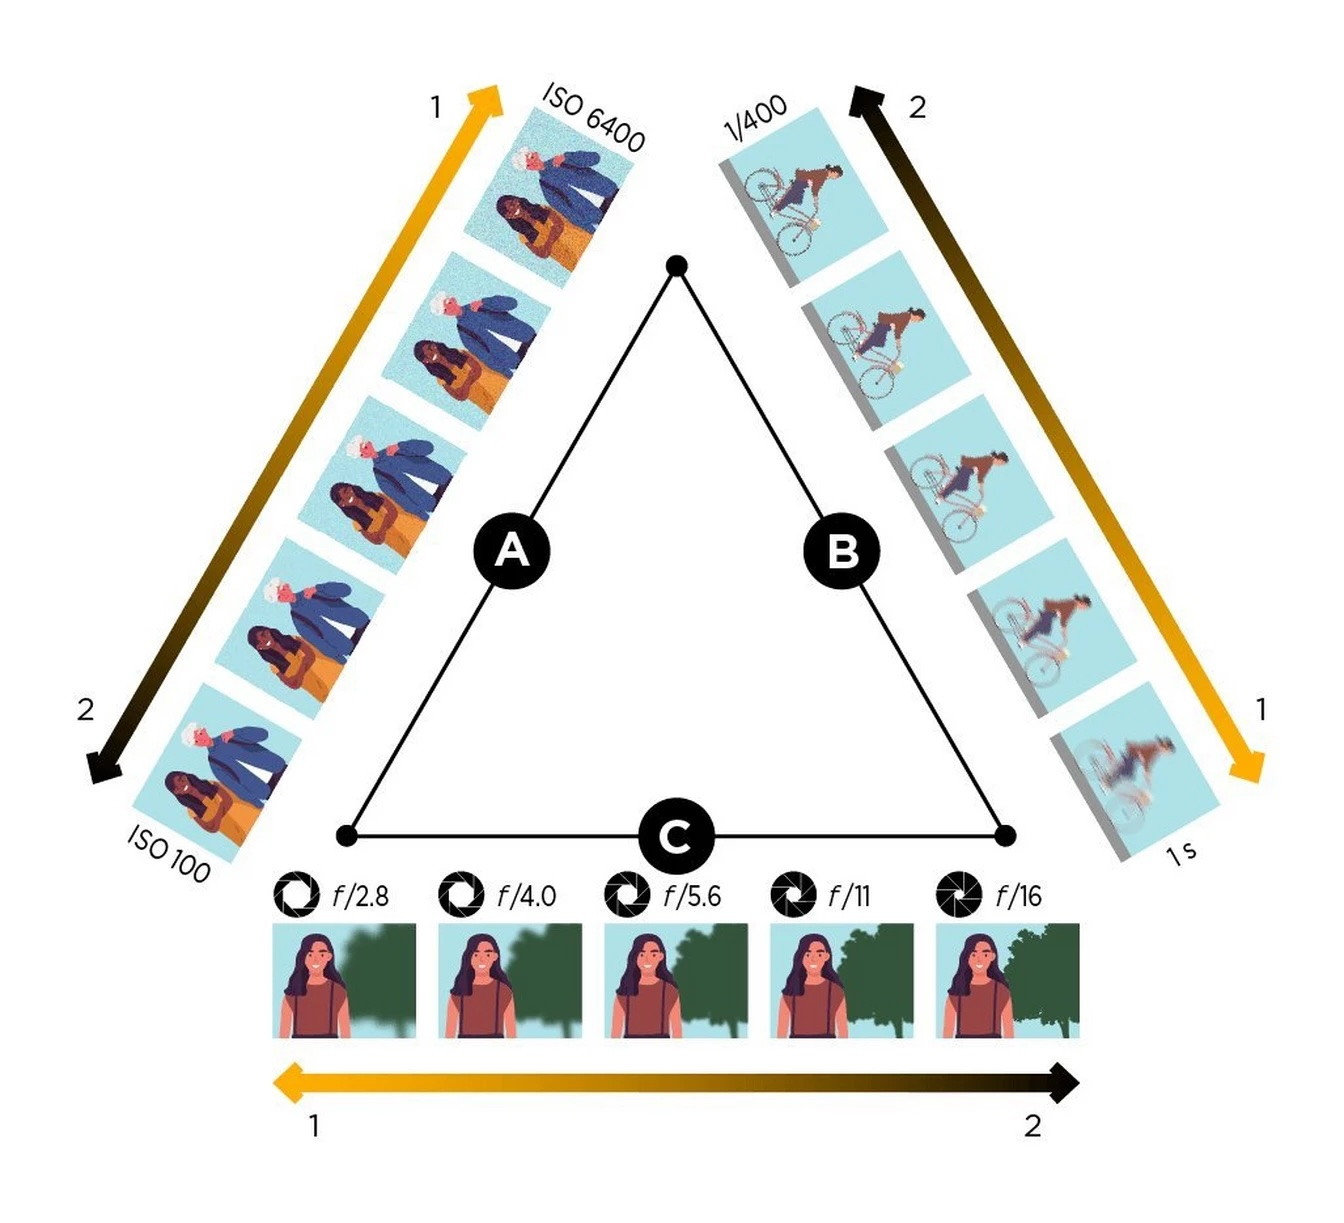
\includegraphics[width=0.8\linewidth]{./img/tradeoffs.jpg}
  \label{fig:tradeoffs}
\end{figure}

\subsubsection{Diaphragm}

In theory, when imaging a scene through a thin lens, only the points at a certain distance can be on focus, all the others appear blurred into circles.
However, as long as the circles are smaller than the size of the photosensing elements (a single pixel), the image will still look on-focus.

\begin{figure}[htbp]
  \centering
  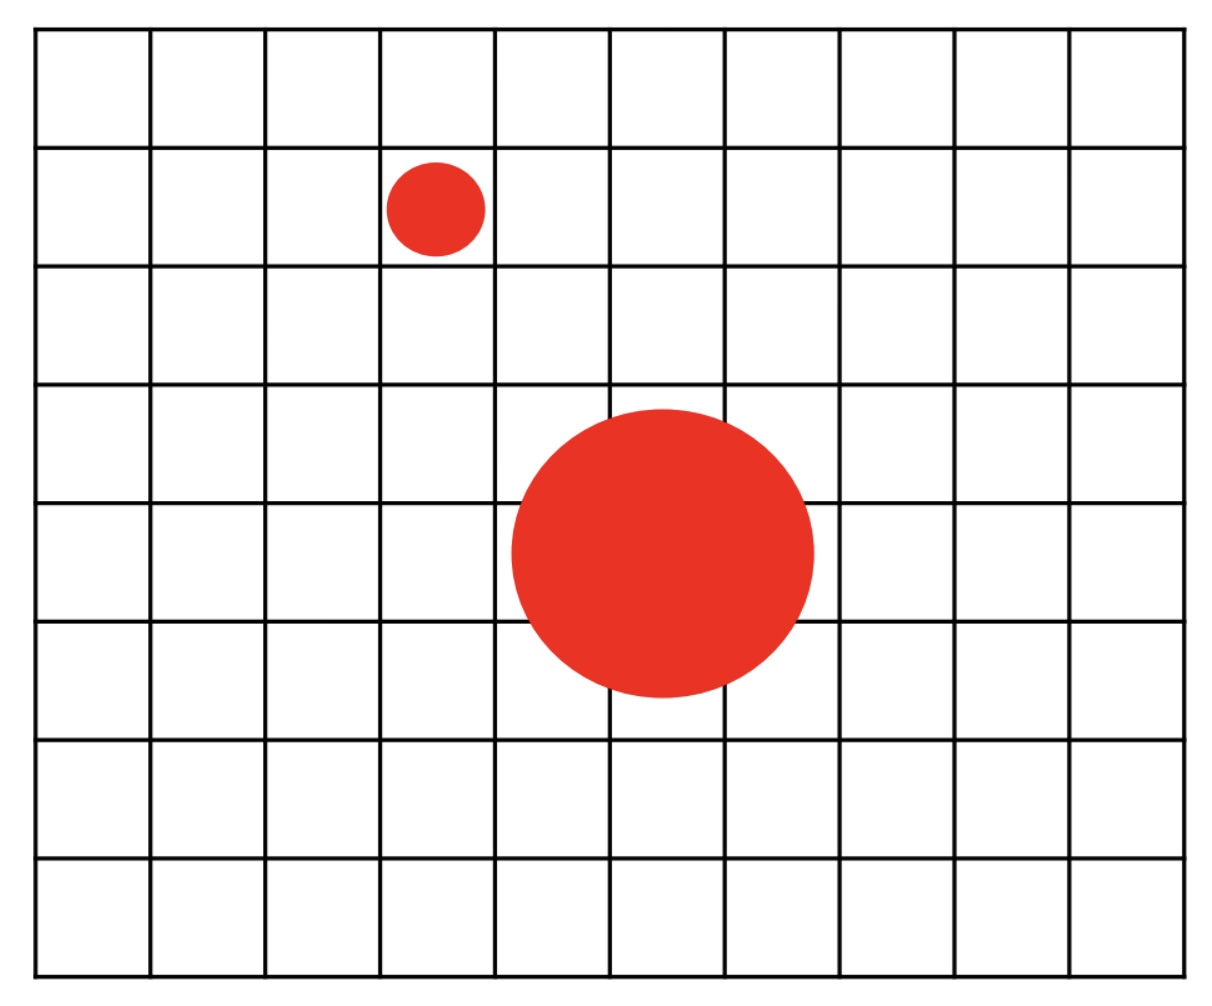
\includegraphics[width=0.55\linewidth]{./img/diaphragm.jpg}
  \caption{Blurring at pixel level}
  \label{fig:diaphragm}
\end{figure}

The range of distances across which the image appears on focus, due to blur circles being small enough, determines the (Depth Of Field) of the imaging apparatus.
Cameras often deploy an adjustable diaphragm (iris) to control the amount of light gathered through the effective aperture of the lens.
\begin{itemize}
  \item Reduce aperture $\rightarrow$ less light $\rightarrow$ smaller blur circle
  \item More aperture $\rightarrow$ more light $\rightarrow$ larger blur circle.
  \item Close the diaphragm $\rightarrow$ increase depth of field $\rightarrow$ not enough light $\rightarrow$ increase exposure time $\rightarrow$ moving object $\rightarrow$ motion blur.
\end{itemize}

\subsubsection{Focusing mechanism (manually changing depth of field)}
To focus on objects at diverse distances we need a mechanism that allows the lens (or the lens subsystem) to translate along the optical axis with respect to the fixed position of the image plane.

\begin{figure}[htbp]
  \centering
  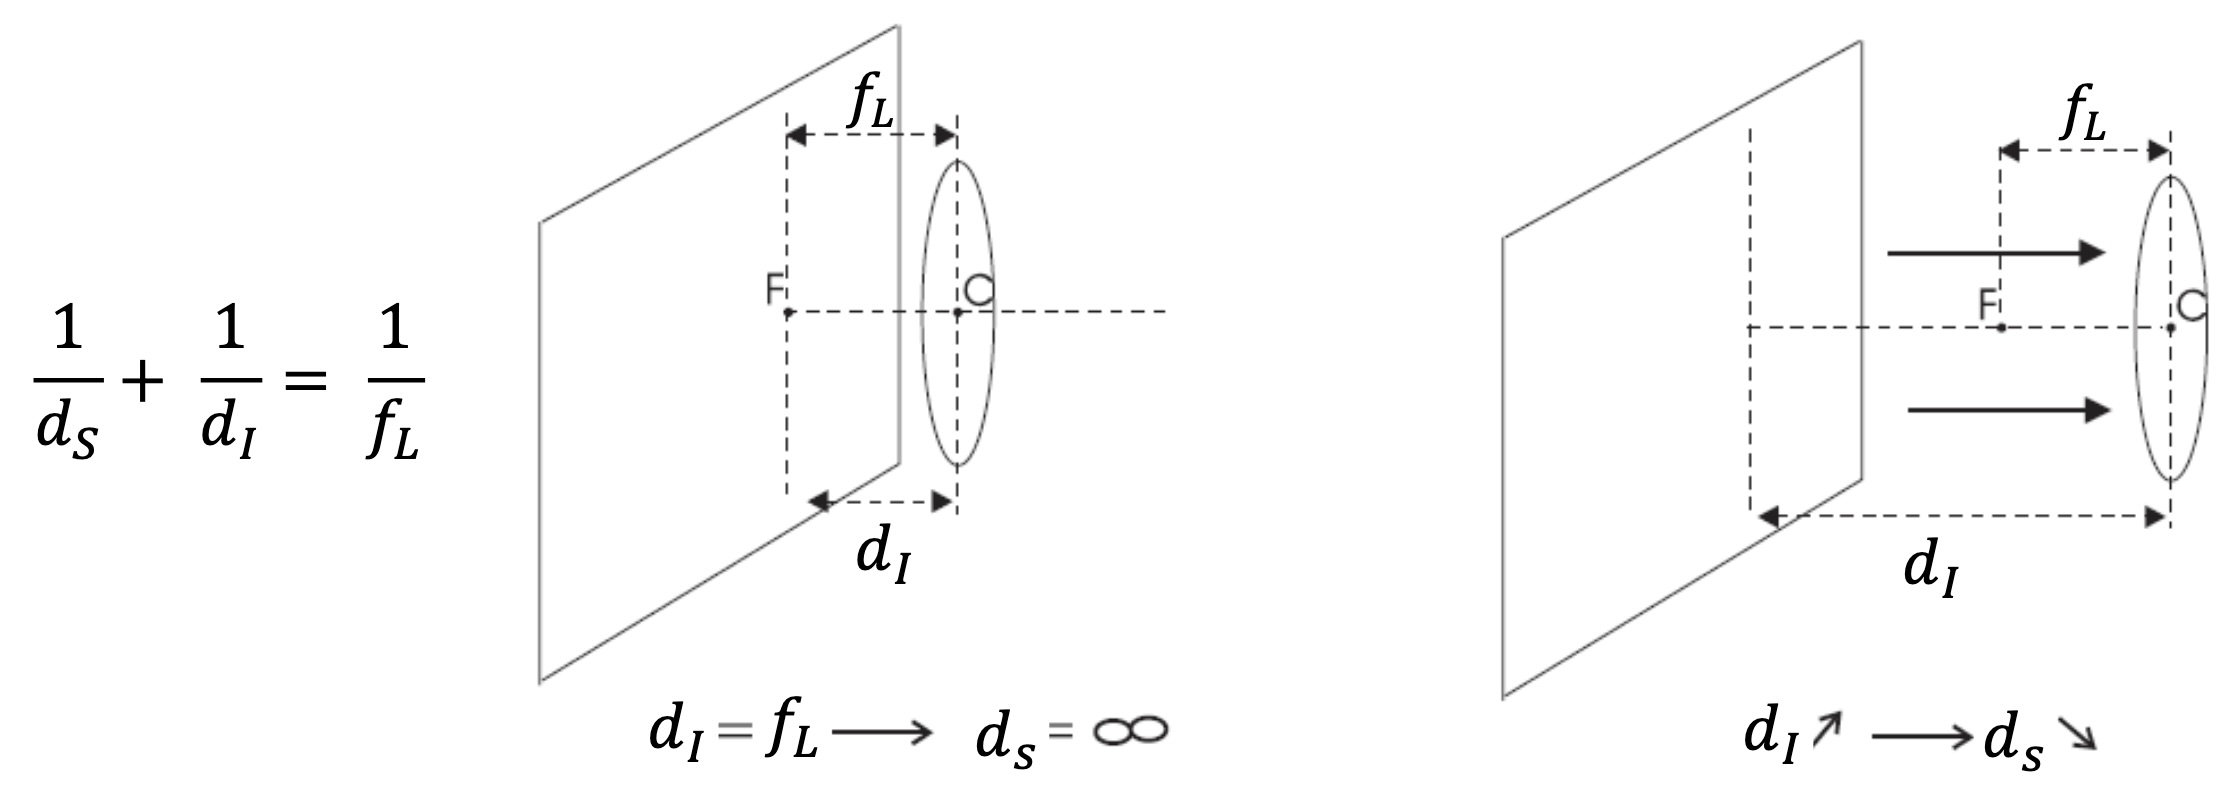
\includegraphics[width=0.7\linewidth]{./img/focusing_mechanism.jpg}
  \caption{Focusing mechanism}
  \label{fig:focusing_mechanism}
\end{figure}

At one end position ($d_I = f_L$) the camera is focused at infinity (objects at inifity are on sharp focus).
The focusing mechanism allows the lens to be translated farther away from the image plane up to a certain maximum value, which determines the minimum focusing distance.

\subsubsection{Image digitization}

How do we convert a continuous image to a discrete one which can be represented on a computer? 
The process can be divided in two steps: sampling and quanitzation.

\begin{figure}[htbp]
  \centering
  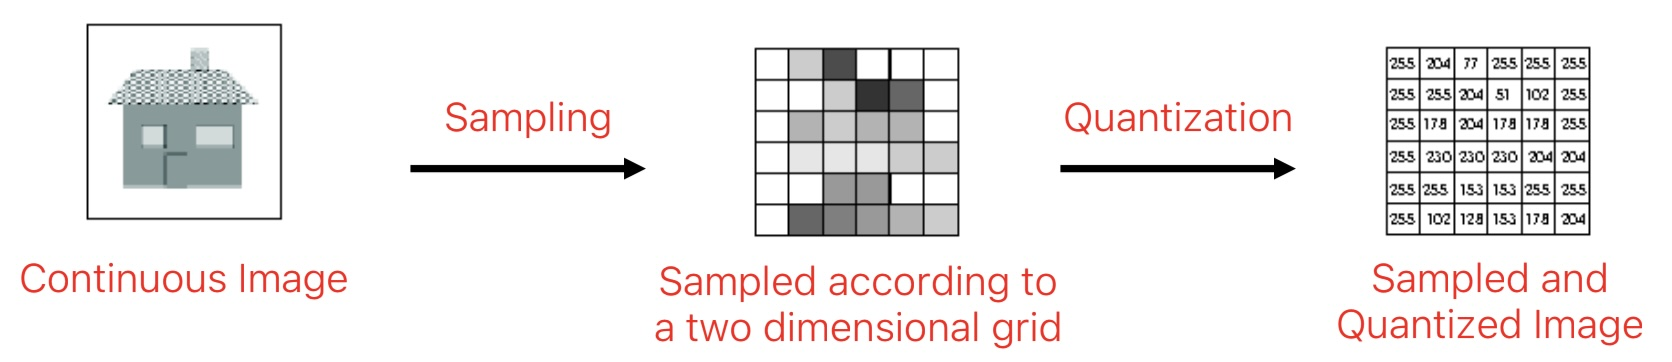
\includegraphics[width=0.55\linewidth]{./img/image_digitization.jpg}
  \caption{The two steps of the image digitization process}
  \label{fig:image_digitization}
\end{figure}

\begin{itemize}
  \item \textbf{Sampling}: the planar continuous image is sampled along both the horizontal and vertical directions to pick up a matrix of $N\times M$ samples (pixels).
  \item \textbf{Quantization}: the continuous range of values associated with pixels is quantized into $l=2^m$ discrete levels known as gray-levels.
  $m$ is the number of bits used to represent a pixel, with the memory occupancy (in bits) of a gray-scale image given by $B = N \times M \times m$. Coloured digital images are typically represented within computers using 3 bytes per pixels. Both more pixels and more bits per pixel result in a higher quality image.
\end{itemize}

The more bits we spend for its representation, the higher the quality of the digital image (it becomes a closer approximation to the ideal continuous image).
This applies both to sampling and quantization.

\subsubsection{Camera sensors}

The sensor is a matrix of photodetectors.
During exposure time, each detector converts the incident light into a proportional electic charge.
The companion circuitry reads-out the charge to generate the output signal, which can be either digital or analog.
For digital cameras the sensor includes the necessary ADC circuitry.

Today, the two main sensor technologies are:
\begin{itemize}
  \item \textbf{Charge Coupled Devices (CCD)}, where the sensor and circuit are separated.
  \item \textbf{ Complementary Metal Oxide Semiconductor (CMOS)}, where everything is on the same circuit.
\end{itemize}

CCD/CMOS sensors can't sense colors, so we place an array of optical filters in front of the photodetectors, to render each pixel sensitive to a specific range of wavelengths.

\subsubsection{SNR}

The intensity measured at a pixel under perfectly static conditions varies due to the presence of random noise.
The main noise sources are:
\begin{itemize}
  \item \textbf{Photon Shot Noise}: the number of photons collected during exposure time is not constant.
  \item \textbf{Electronic Circuitry Noise}: generated by the electronics.
  \item \textbf{Quantization Noise}: related to the ADC conversion.
  \item \textbf{Thermal Noise (Dark Current Noise)}: random charge observed due to thermal excitement.
\end{itemize}

SNR can be expressed both in decibels and bits.

\subsubsection{Dynamic Range (DR)}
If the sensed amount of light is too small, the "true" signal cannot be distinguished from noise.
Given $E_{\text{min}}$: the minimum detectable irradiation, and $E_{\text{max}}$, the saturation irradiation.
The Dynamic Range (DR) of a sensor is defined as $DR = \frac{E_{\text{max}}}{E_{\text{min}}}$, and like the SNR, it is often specified in decibels or bits.

Like SNR, the higher the DR the better it is.
A \textbf{higher DR} corresponds to the ability of the sensor to simultaneously \textbf{capture in one image both the dark and bright} structures of the scene.

% lecture 2 part 2
\subsection{Image Filtering}

\subsubsection{Noise and image filters}

In computer vision we have to deal with noise.
Noise is always different, and more noticeable in uniform regions of the image.
The simplest thing to reduce noise is to output the average of the pixel color over time, to get \textbf{almost} the ideal noiseless value.
$$O(p) = \frac{1}{T} \sum_{t=1}^{T} I_k(p) = \frac{1}{T} \sum_{t=1}^{T}(\tilde{I}(p) + n_t(p))$$

This technique works well on still images.

\begin{figure}[htbp]
  \centering
  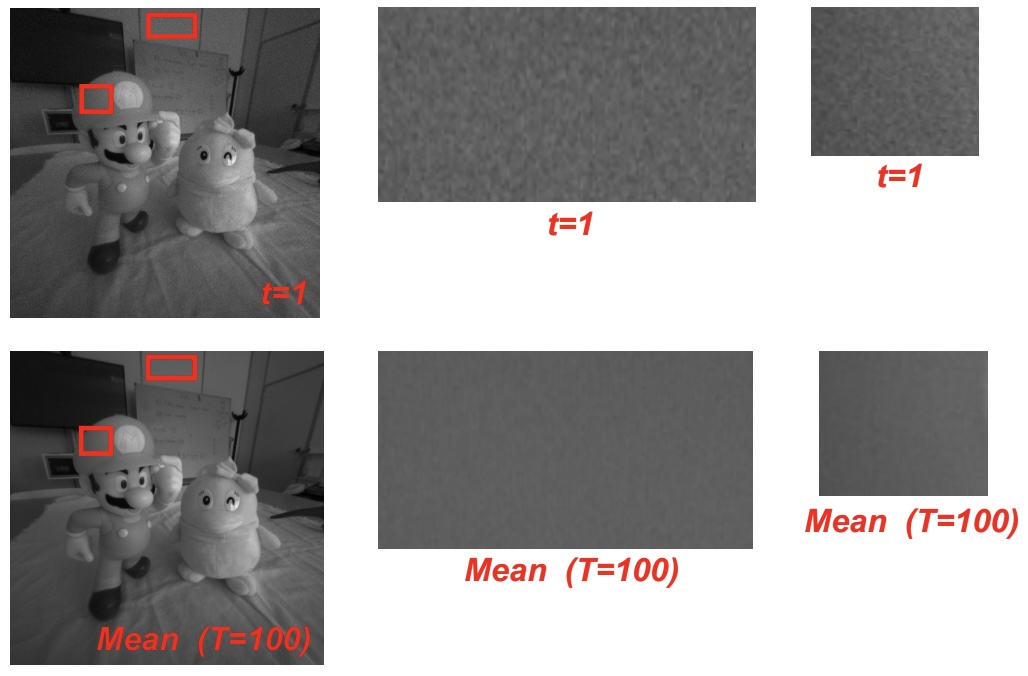
\includegraphics[width=0.7\linewidth]{./img/denoising_simple.jpg}
  \caption{Simple denoising}
  \label{fig:denoising_simple}
\end{figure}

If we are given a simple image, we may compute a mean across neighbouring pixels, like a spatial rather than temporal mean.
The size of the square of the neighbouring pixels is a tradeoff.

This is a very basic denoising filter.

Image filters are image processing operators that compute the new intensity (colour) of a pixel, $p$, based on the intensities (colours) of those belonging to a neighbourhood (support) of $p$.

\subsubsection{Convolution}

An important sub-class of filters is given by \textbf{Linear} and \textbf{Translation-Equivariant (LTE)} operators.

The \textbf{application of filters} in image processing consists in a \textbf{2D convolution} between the input image and the impulse response function of the LTE operator.

LTE operators are used as feature extractors in Convolutional Neural Networks (CNNs).

Given an input 2D signal $i(x,y)$, a 2D operator $T{i(x,y)}$ is said to be linear if and only if
$$ T\{\alpha i_1(x,y) + \beta i_2(x,y)\} = \alpha o_1(x,y) + \beta o_2(x,y) $$ with $o_1 = T{i_1}$ and $o_2 = T{i_2}$ and $\alpha, \beta$ are two constants.
The operator is said to be \textbf{translation-equivariant} if and only if: $T\{i(x-x_0, y-y_0)\} = o(x-x_0, y-y_0)$

If the operator is LTE, the output signal is given by the \textbf{convolution} between the input signal and the impulse response (point spread function) $h(x,y) = T{\delta (x,y)}$.

$$o(x,y) = i(x,y) * h(x,y) = T\{i(x,y)\}$$

$$i(x,y) * h(x,y) = \int_{-\infty}^{\infty} \int_{-\infty}^{\infty} i(\alpha, \beta) h(x-\alpha, y-\beta) \, d\alpha  d\beta $$

\begin{figure}[htbp]
  \centering
  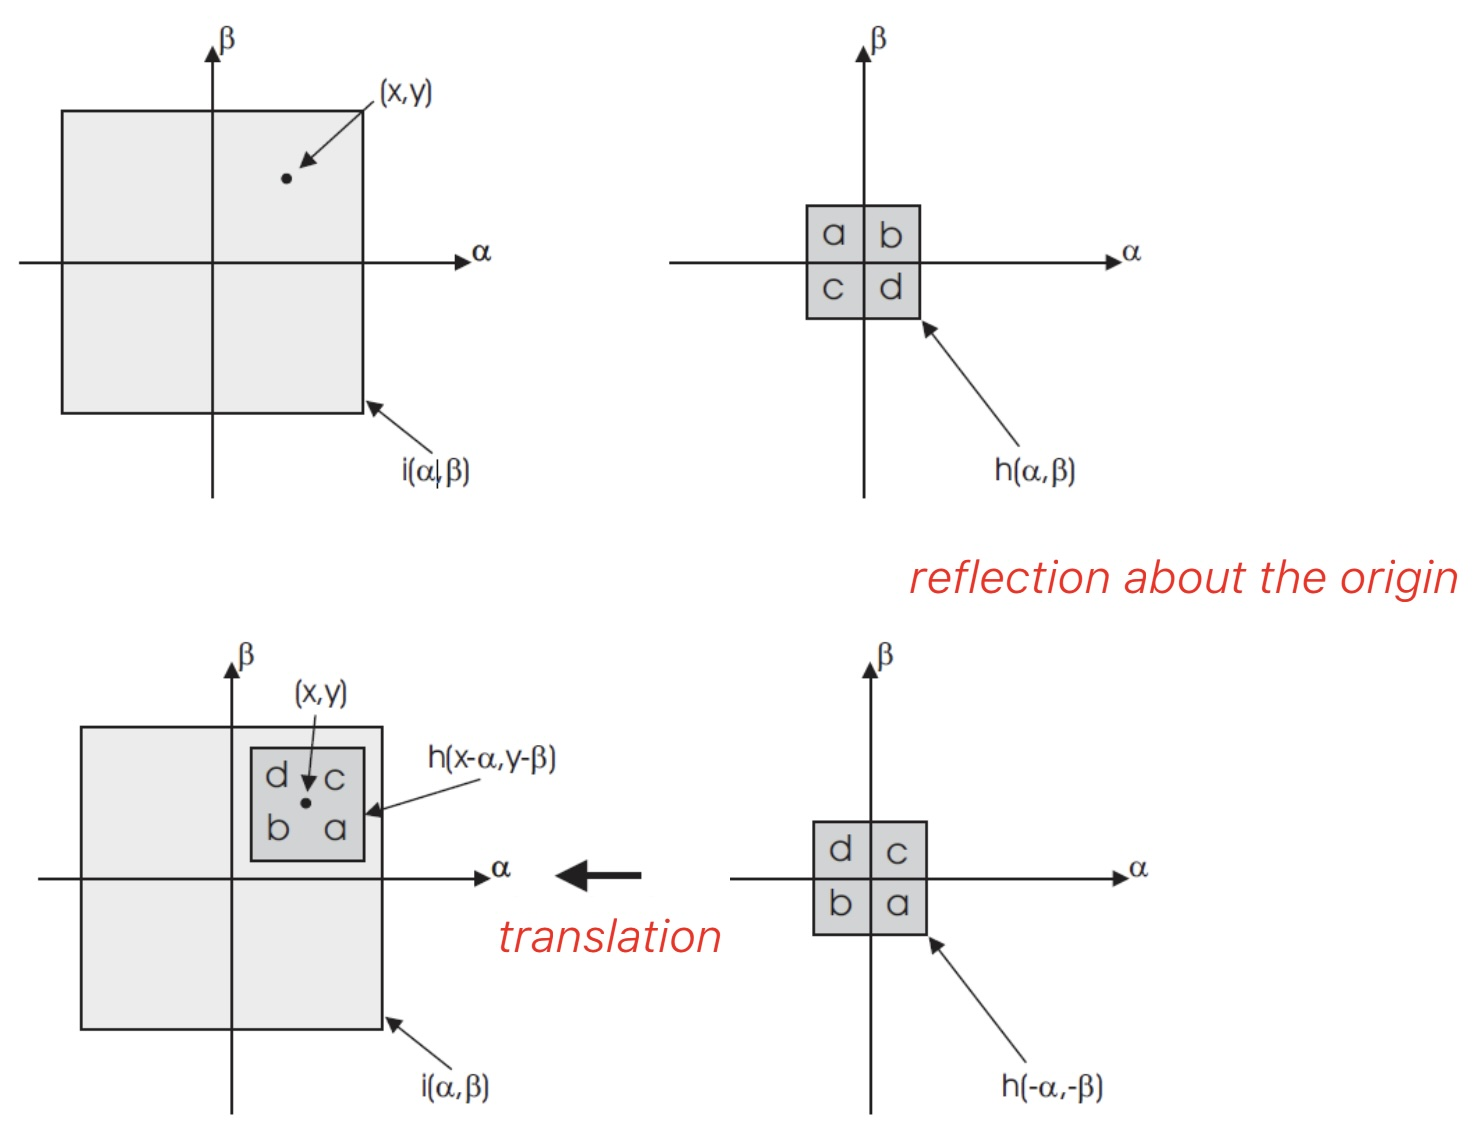
\includegraphics[width=0.6\linewidth]{./img/graphical_convolution.jpg}
  \caption{A graphical view of convolution}
  \label{fig:graphical_convolution}
\end{figure}

Convolutions have some useful properties:
\begin{itemize}
  \item \textbf{Associative property}: $f * (g * h) = (f*g)*h$ (useful because we can decompose kernels and obtain faster operations).
  \item \textbf{Commutative property}: $f*g = g*f$.
  \item \textbf{Distributive property}: $f*(g+h) = f*g + f*h$.
  \item \textbf{Convolution commutes with differentiation}: $(f*g)' = f'*g = f*g'$.
\end{itemize}

The correlation of signal $i(x,y)$  with respect to signal $h(x,y)$ is defined as:
$$i(x,y) \circ h(x,y) = \int_{-\infty}^{\infty} \int_{-\infty}^{\infty} i(\alpha, \beta) h(x-\alpha, y-\beta) \, d\alpha  d\beta $$

Correlation is not commutative, unlike the convolution.

\subsubsection{Discrete convolution}

Normal convolution is useful for signal theory, but we want to have a discrete convolution, where we use summations instead of integrals.
The four convolution properties highlighted for the convolution hold for the discrete one too.

\subsubsection{Practical implementation}
CNNs learn flipped kernels.
In image processing both the the input image and the kernel are stored into matrices of given finite sizes, with the image being much larger than the kernel.
Conceptually, to obtain the output image we need to slide the kernel across the whole input image and compute the convolution at each pixel.

We have an issue on borders, since the kernel "goes out" of the matrix of the image.
We have two main options to solve this issue:
\begin{itemize}
  \item \verb|CROP|: common in image processing.
  \item \verb|PAD|: preferred in CNNs. We can do zero-padding, replicate the first pixel many times, reflect the first $k$ pixels (half of the kernel)...
\end{itemize}

Without padding convolutions shrink the images.

\begin{figure}[htbp]
  \centering
  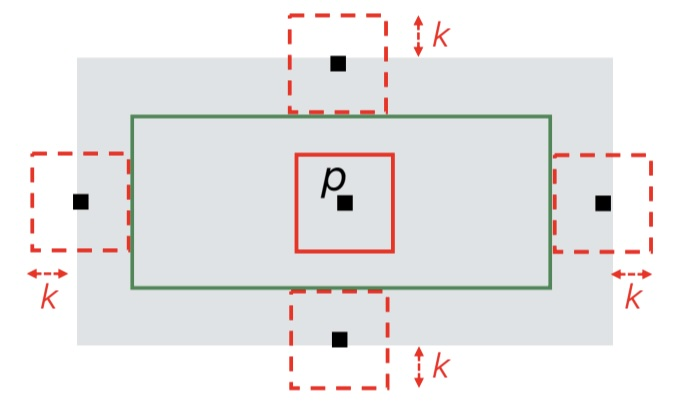
\includegraphics[width=0.7\linewidth]{./img/convolution_visualization.jpg}
  \caption{Issues with convolutions}
  \label{fig:convolution_visualization}
\end{figure}

\subsubsection{Mean filter}

\textbf{Mean filtering} is the \textbf{simplest and fastest way to denoise an image}.
It consists in replacing each pixel intensity by the average intensity overa chosen neighbourhood.
According to signal processing theory, \textbf{the Mean Filter carries out a low-pass filtering operation}, which in image processing is \textbf{also referred to as image smoothing}.
Smoothing is often aimed at image denoising, but sometimes is used to cancel out small-size unwanted details that might hinder the image analysis task.
Linear filtering \textbf{reduces noise but blurs the image}, so we lose sharpness.

% lecture 3
\subsubsection{Gaussian filter}

The Gaussian filter is an LTE operator whose impulse response is a 2D Gaussian function.

\begin{figure}[htbp]
  \centering
  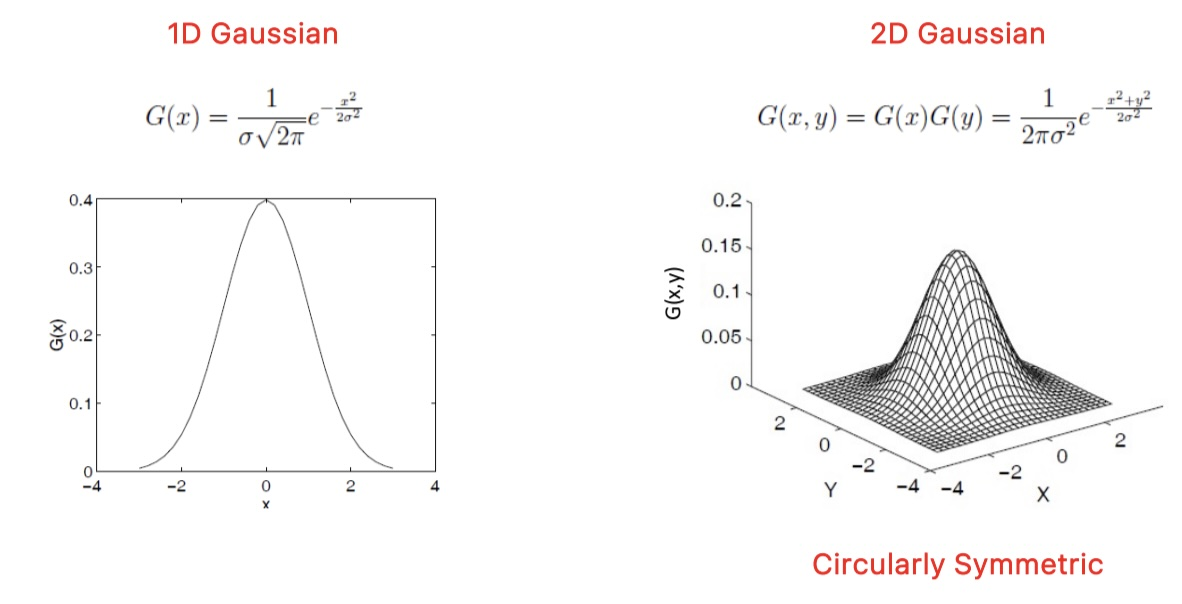
\includegraphics[width=0.7\linewidth]{./img/gaussian_filter.jpg}
  \caption{1D and 2D Gaussian plot}
  \label{fig:gaussian_filter}
\end{figure}

The larger the size of the gaussian kernel, the more accurate the approximation will be, but the computational cost grows with the filter size.
We should then use larger sizes for filters with higher $\sigma$, smaller sizes whenever $\sigma$ is smaller.
A typical rule is to choose the size of the filter by capturing the interval $[-3\sigma, +3\sigma]$ since it captures 99\% of the energy of the Gaussian impulse.
% The Gaussian filter is the only one which has been mathematically proven of not altering image information but just semplification.
To speedup the filtering we can apply the 2D gaussian by doing 2 1D gaussian filterings.

We also observe that the higher the $\sigma$, the higher is the smoothing caused by the filter.
We can use this filter to remove details from the image.

\subsubsection{Median filter}

There is noise that Gaussian filters can't handle well, that is the salt and pepper noise. It's usually caused by image corruption (or broken pixels in the sensor).
Linear filtering is ineffective and just blurs the image.

We can use a \textbf{non-linear filter}, where each pixel intensity is replaced by the \textbf{median over a given neighbourhood}.
Median filtering counteracts impulse noise effectively, since \textbf{outliers tend to fall at either the top or the bottom end of the sorted intensities}.
Median filtering tends to keep sharper edges than linear filters such as the Mean or the Gaussian.

\begin{figure}[htbp]
  \centering
  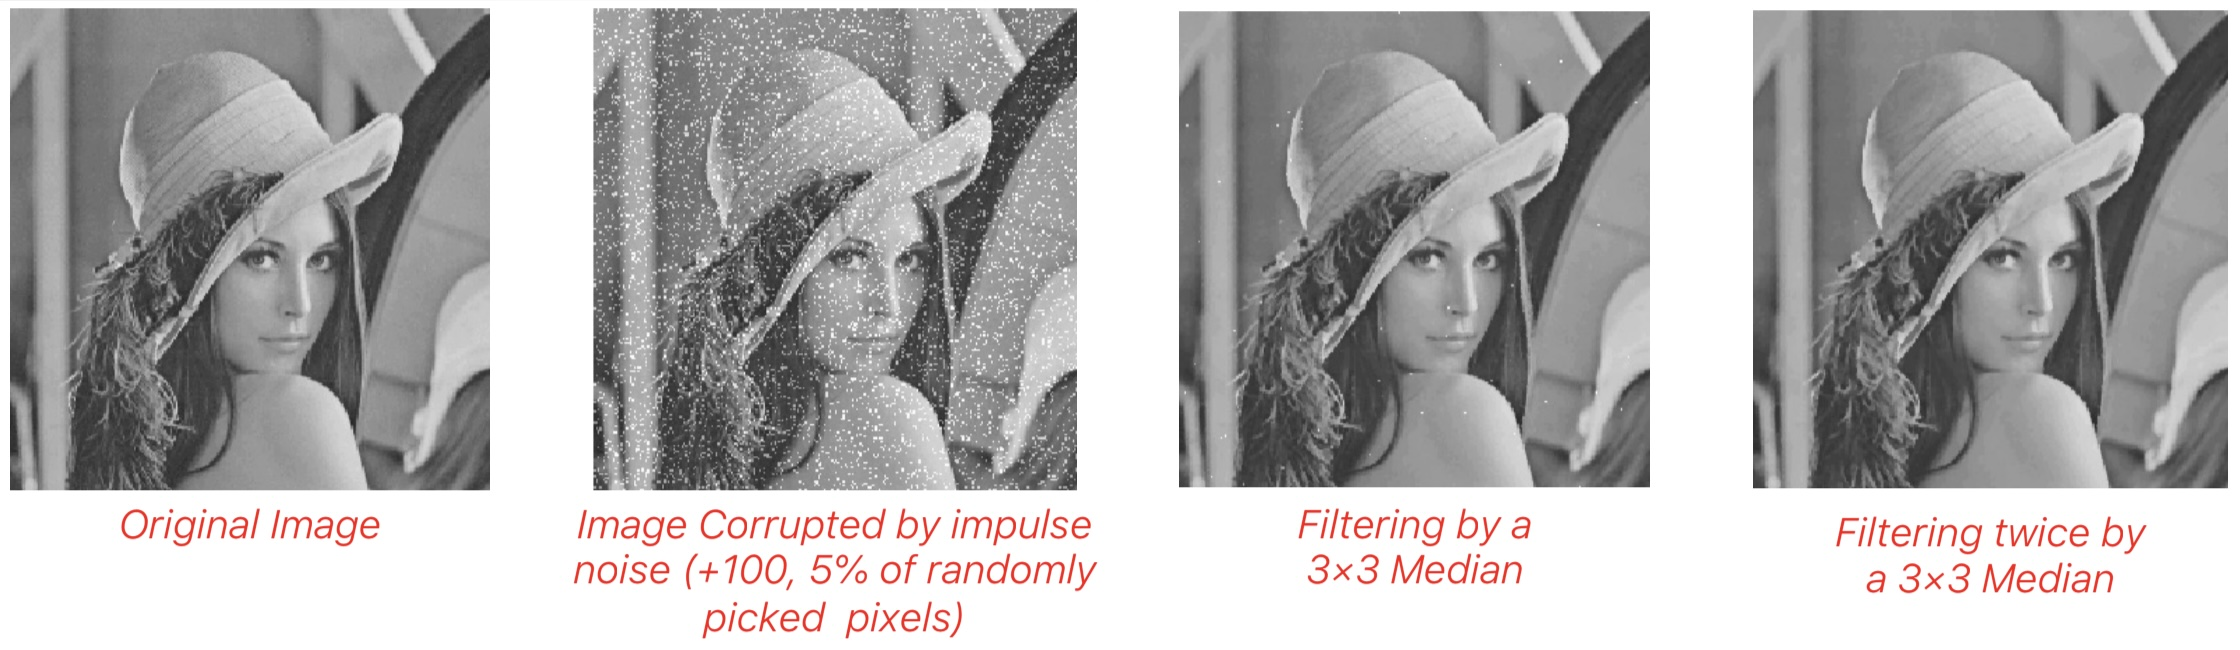
\includegraphics[width=0.9\linewidth]{./img/median_filter_application.jpg}
  \caption{Example of the power of the median filter}
  \label{fig:median_filter_application}
\end{figure}

The median filter can effectively denoise the image without introducing significant blur, yet, Gaussian-like noise, such as sensor noise, cannot be dealt with by the median, as this would require computing new noiseless intensities.

\subsubsection{Bilateral filter}

The bilateral filter preserves edges while filtering out noise.
It's an advanced non-linear filter to accomplish \textbf{denoising of Gaussian-like noise without blurring the image}.
It's also called edge preserving smoothing.

$$O(p) = \sum_{q\in S} H(p,q) \cdot I_q \,\,\,\,\,\,\,\, H(p,q) = \frac{1}{W(p)} G_{\sigma_s}(d_s(p,q))G_{\sigma_r}(d_r(p,q))$$

\begin{itemize}
  \item \textbf{spatial distance}: $d_s(p,q) = ||p-q||_2 = \sqrt{(u_p - u_q)^2 + (v_p - v_q)^2}$.
  \item \textbf{range (intensity) distance}: $d_r(I_p, I_q) = |I_p - I_q|$.
  \item \textbf{normalization factor}: $W(p) = \sum_{q \in S} G_{\sigma_s}(d_s(p,q))G_{\sigma_r}(d_r(p,q))$
\end{itemize}

\begin{figure}[htbp]
  \centering
  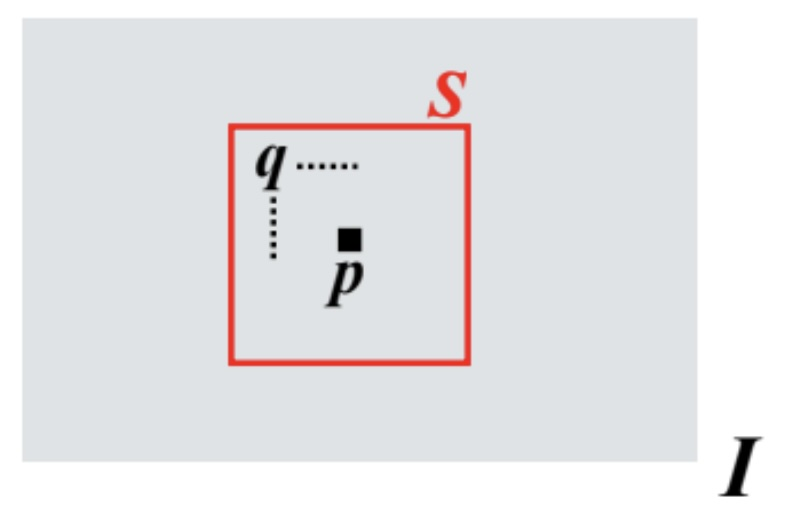
\includegraphics[width=0.5\linewidth]{./img/bilateral_filter_application.jpg}
  \caption{Application of the bilateral filter}
  \label{fig:bilateral_filter_application}
\end{figure}

Given the supporting neighbourhood, neighbouring pixels take a larger weight as they are both closer and more similar to the central pixel.
At a pixel nearby an edge, the neighbourhood falling on the oter side of the edge looks quite different and thus cannot contribute significantly to the output value due to their weights being small.
\textbf{The kernel has to be recomputed for each pixel}.

\begin{figure}[htbp]
  \centering
  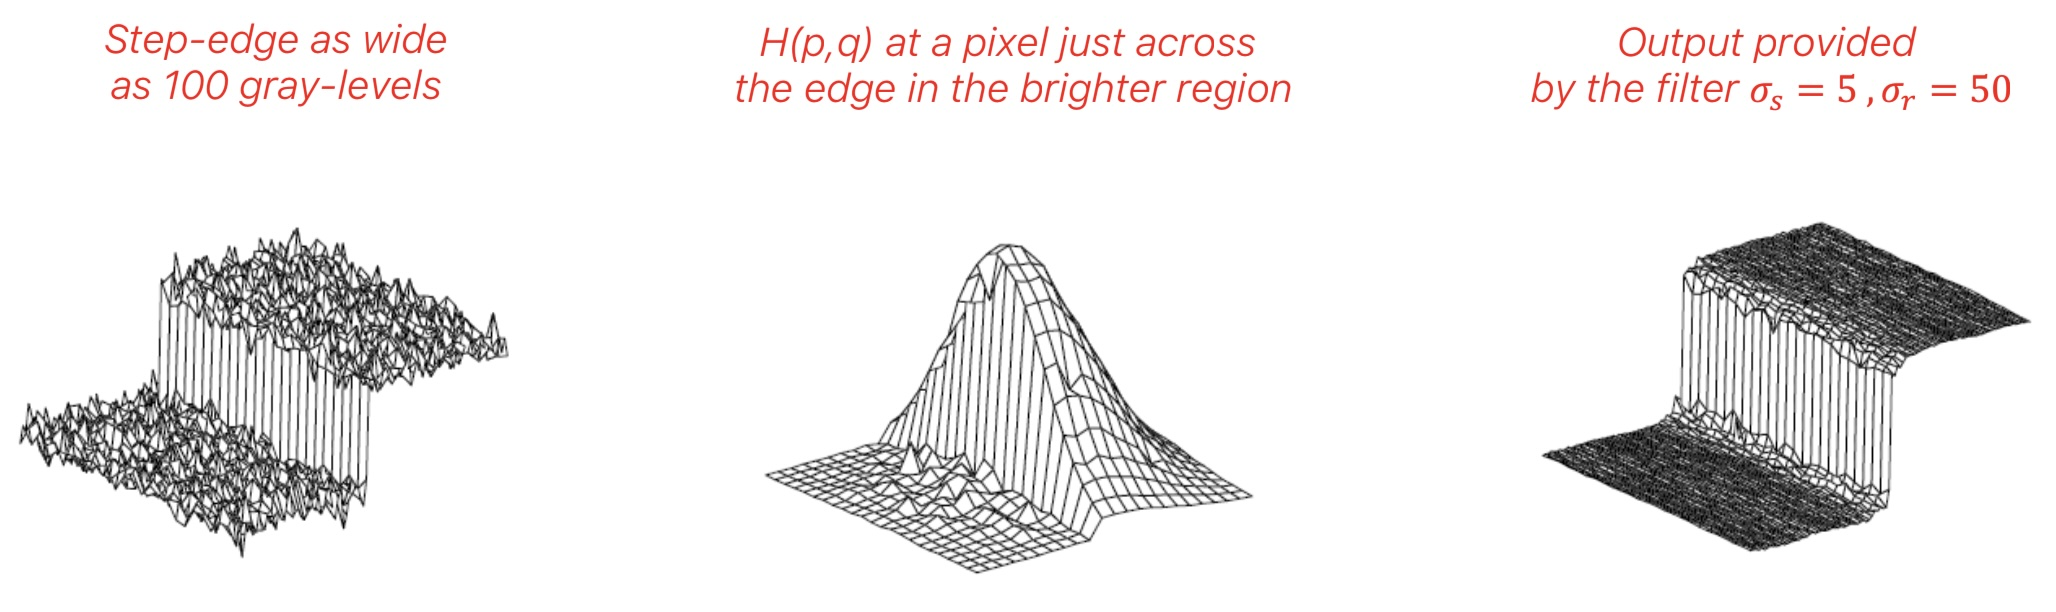
\includegraphics[width=0.9\linewidth]{./img/bilateral_filter.jpg}
  \caption{Bilateral filter differences}
  \label{fig:bilateral_filter}
\end{figure}

\subsubsection{Non-local means filter}

It's another non-linear edge preserving smoothing filter.
The key idea is that the \textbf{similarity among patches spread over the image} can be deployed to achieve denoising.
It's even more expensive than the bilateral filter, since it has to look at more of the image.

\begin{figure}[htbp]
  \centering
  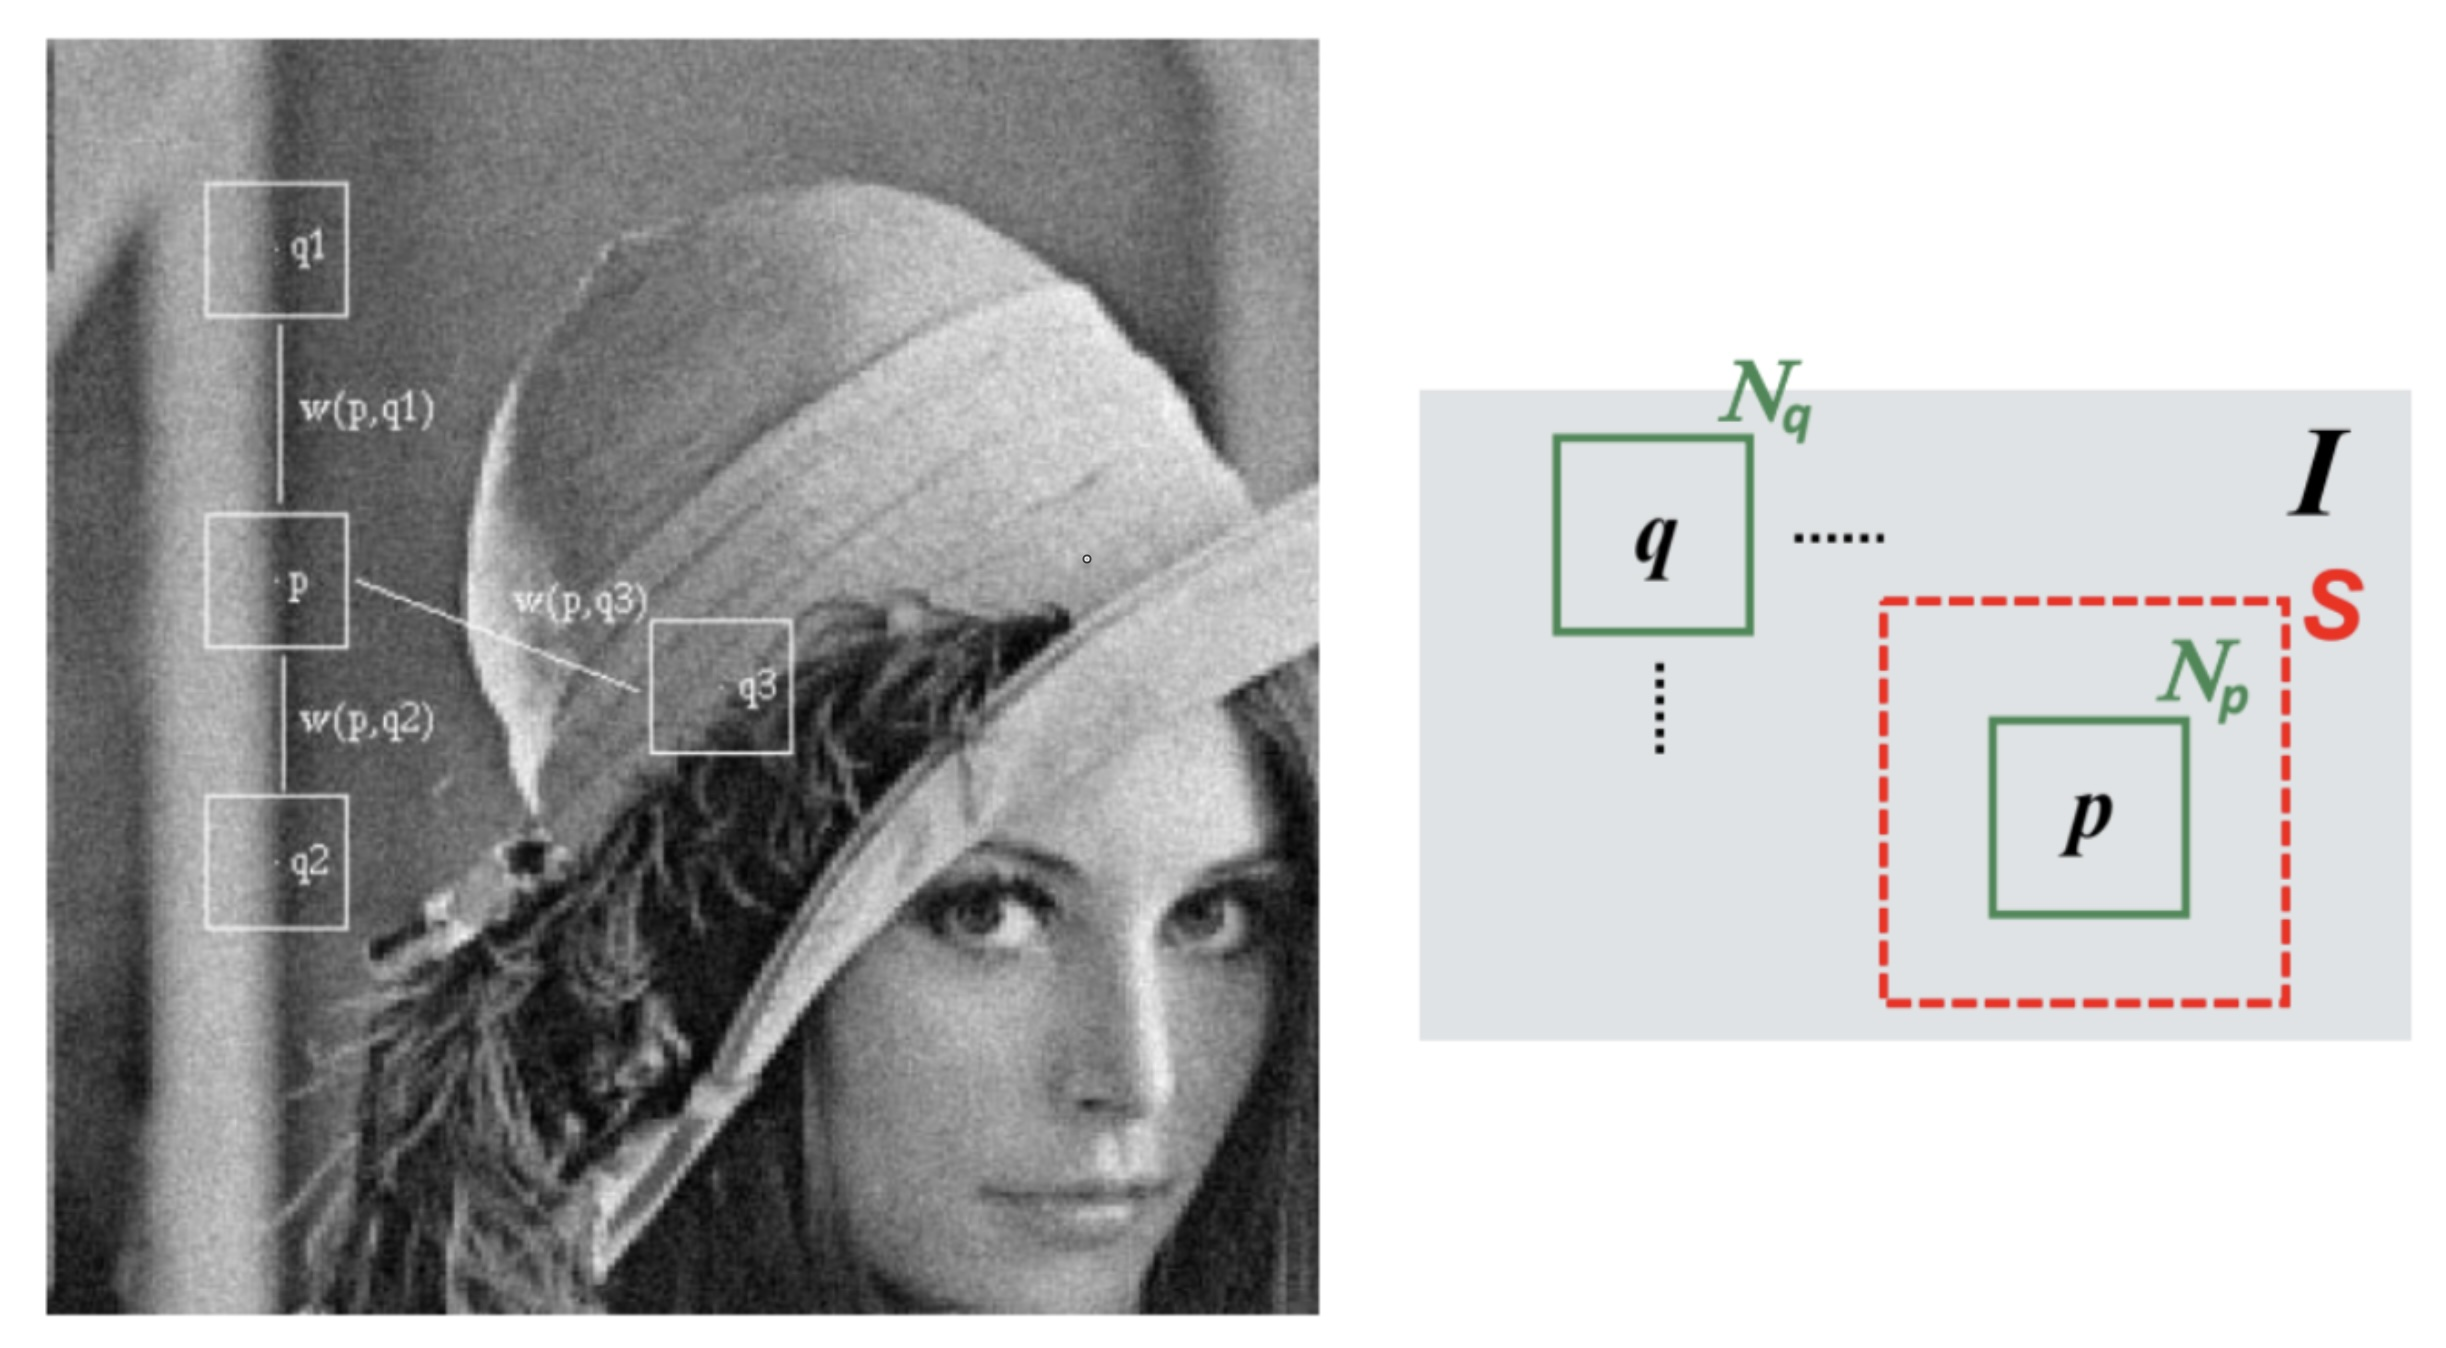
\includegraphics[width=0.7\linewidth]{./img/nonlocalmeans_filter.jpg}
  \caption{Non-local means filter}
  \label{fig:nonlocalmeans_filter}
\end{figure}

\begin{figure}[htbp]
  \centering
  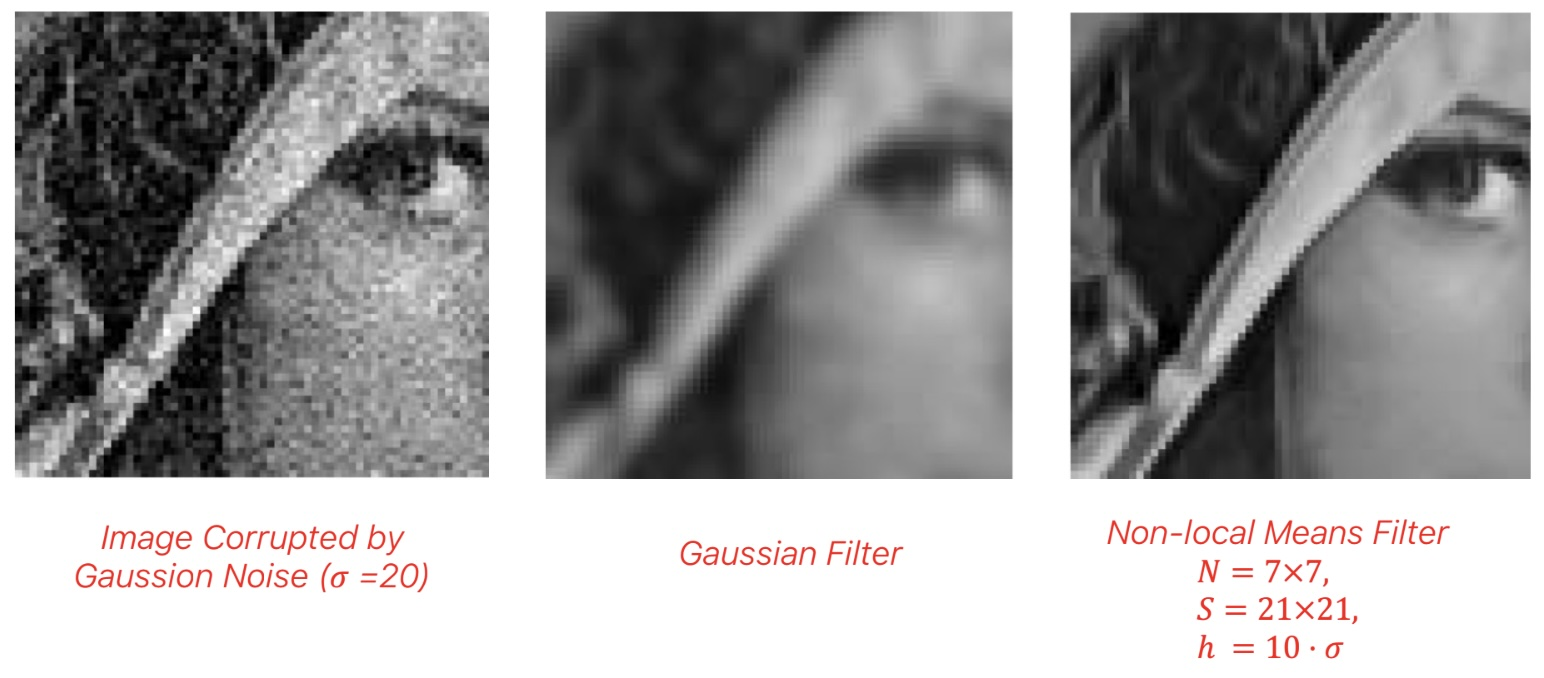
\includegraphics[width=0.7\linewidth]{./img/nonlocalmeans_comparison.jpg}
  \caption{Difference between Gaussian filter and non-local means filter}
  \label{fig:nonlocalmeans_comparison}
\end{figure}

\subsection{Edge detection}

Edge points are local features of the image that capture important information related to its semantic content.
Edges are pixels that lie exactly in between image regions of different intensities.

\paragraph{1D step-edge}
We can detect an edge with a sharp change of a 1D signal (1D step-edge).
The simplest edge-detection operator relies on thresholding the absolute value of the derivative of the signal.

\paragraph{2D step-edge}
A 2D step-edge is characterized not only by its strength but also by its direction (diagonal edge).
The operator which allows us to sense the edge in any direction is the gradient:
$$\nabla I(x,y) = \frac{\partial I(x,y)}{\partial x}i + \frac{\partial I(x,y)}{\partial y}j$$
The \textbf{gradient tells the direction along which the function exhibits its maximum variation}.
We can use differences to approximate the gradient (since we are in the discrete world and we talk about pixels, not functions).
We can estimate the magnitude of the gradient by using different approximations.
We choose $|\nabla I|_{\max}=\max(|I_x|, |I_y|)$, since it's fast and invariant with respect to the edge direction.

\paragraph{Edges and noise}
In real images an edge will not look as smooth as we have seen due to noise.
Taking derivatives of noisy signals is an ill posed problem (the solution is not robust with respect to the input variation) since derivatives amplify noise.
Noise robustness is usually achieved by smoothing the signal before computing the derivatives required to highlight edges.
Smoothing has the side effect of blurring true edges, making it more difficult to detect and localize them, since pixel of different colors will look similar after filtering because of the blending.

\paragraph{Prewitt and Sobel}
% We might wish to approximate partial derivatives by central differences.
% This is done to average around the point because if we are on an edge around us there is a big transition.
% Likewise, the central pixel can be weighted more (the center pixel should be more important).
Prewitt and Sobel address the challenge of detecting edges in noisy environments by combining smoothing and differentiation into a single step.
The Prewitt and Sobel operators perform spatial filtering by using $3 \times 3$ convolution kernels.
Each kernel smooths the image in one direction (reducing noise) and computes the derivative in the perpendicular region (highlighting edges).
Both operators use two kernels: one detects vertical edges, and one horizontal ones.
After convolving the image with both kernels, the gradient magnitude and direction are computed.

$$\text{Magnitude} = \sqrt{G_x^2 + G_y^2} \quad\quad \text{Direction} = \arctan(\frac{G_y}{G_x})$$

Prewitt is better for precise edge localization in cleaner images.
Sobel is preferable in noisy images but may slightly blur edges.


\subsubsection{Non-Maxima Suppression (NMS)}

Detecting edges by gradient thresholding is inherently inaccurate, since \textbf{it's difficult to choose the right threshold} a priori.
A better approach to detect edges may consist in finding the local maxima of the absolute value of the derivative of the signal.

When dealing with 2D images, we should look for:
\begin{itemize}
  \item Maxima of the absolute value of the derivative (gradient magnitude).
  \item Along the gradient direction (orthogonal to the edge direction).
\end{itemize}

We don't know in advance the correct direction to carry out Non-Maxima Suppression (NMS).
The direction has to be estimated locally based on the gradient's direction.
The magnitude of the gradient has to be estimated at points which do not belong to the discrete pixel grid.
Such values can be estimated by linear interpolation of those computed at the closest point belonging to the grid.

A final thresholding step on the magnitude of the gradient at the points selected by the NMS process typically helps pruning out unwanted edges due to either noise or less important details.

\subsubsection{Canny's edge detector}
Canny proposed to set forth quantitative criteria to measure the performance of an edge detector and then to find the optimal filter with respect to such criteria.
The three criteria he proposed were:
\begin{itemize}
  \item \textbf{Good detection}: correctly extract edges in noisy images.
  \item \textbf{Good localization}: distance between found and true edge should be minimum.
  \item \textbf{One response to one edge}: detect one single edge pixel at each true edge.
\end{itemize}

A straightforward Canny edge detector can be achieved by:
\begin{itemize}
  \item Gaussian smoothing.
  \item Gradient computation.
  \item NMS along the gradient direction.
\end{itemize}

2D convolution by a Gaussian can be slow, so we can leverage on separability of the Gaussian function to speedup the calculation: $G(x,y) = G(x)G(y)$.

Non Maxima-Suppression (NMS) is often followed by thresholding of gradient magnitude to help distinguish between true "semantic" edges and unwanted ones.
Edge \textbf{streaking} may occur when magnitude varies along object contours.

Canny proposed a "hysteresis" thresholding approach relying on a higher $T_h$ and a lower $T_l$ threshold.
A pixel is taken as an edge if either the gradient magnitude is higher than $T_h$ or higher than $T_l$ and the pixel is a neighbor of an already detected edge.

The hysteresis thresholding is usually carried out by tracking edge pixels along contours.
First the edge candidates are provided by NMS, then all strong edges are picked, and then for each strong edge we track the weak edges along contours.

\paragraph{Zero-crossing}
Instead of maximum values we can look for zero-crossing of the second derivative of the signal to locate edges (instead of the peaks of the first derivative).
This requires significant computational effort since we are calculating second derivatives.

\subsubsection{Second derivative along the gradient \& Laplacian}
The second derivative along the gradient's direction can be obtained as $n^THn$.

\begin{itemize}
  \item \textbf{Unit vector along the gradient's direction} $n = \frac{\nabla I(x,y)}{||\nabla I(x,y)||}$
  \item \textbf{Hessian matrix} $H =  \begin{bmatrix} \frac{\partial^2 I(x,y)}{\partial x^2} & \frac{\partial^2 I(x,y)}{\partial x \partial y} \\ \frac{\partial^2 I(x,y)}{\partial y \partial x} & \frac{\partial^2 I(x,y)}{\partial x^2} \end{bmatrix} $
\end{itemize}

Computing the second derivative along the gradient turns out very expensive.

\paragraph{Discrete Laplacian}
We can use the forward and backward differences to approximate first and second order derivatives.
It can be shown that the zero-crossing of the Laplacian typically lay close to those of the second derivative along the gradient.
Yet, the former differential operator is much faster to compute.

\subsubsection{Laplacian of Gaussian (LoG)}
A robust edge detector should include a smoothing step to filter out noise.
Edge detection by using the Laplacian of Gaussian (LoG) can be summarized as follows:
\begin{itemize}
  \item \textbf{Gaussian smoothing}: $\tilde{I}(x,y) = I(x,y) * G(x,y)$.
  \item \textbf{Second order differentiation} by the Laplacian.
  \item Extraction of the \textbf{zero-crossing} of $\nabla^2 \tilde{I}(x,y)$
\end{itemize}

Practical implementations of the LoG may deploy the properties of convolutions to speed-up the computation.

We can find sign changes from minus to plus (and viceversa) between two consecutive pixels.
Once a sign change is found, the actual edge may be localized:
\begin{itemize}
  \item At the pixel where the LoG is positive (darker side of the edge)
  \item At the pixel where the LoG is negative (brighter side of the edge)
  \item At the pixel where the \textbf{absolute} value of the LoG is smaller (it's the best choice, since the edge turns out closer to the true zero-crossing).
\end{itemize}

Using a \textbf{higher $\sigma$ yields less details}, so usually we use it for noisy images.

\begin{figure}[htbp]
  \centering
  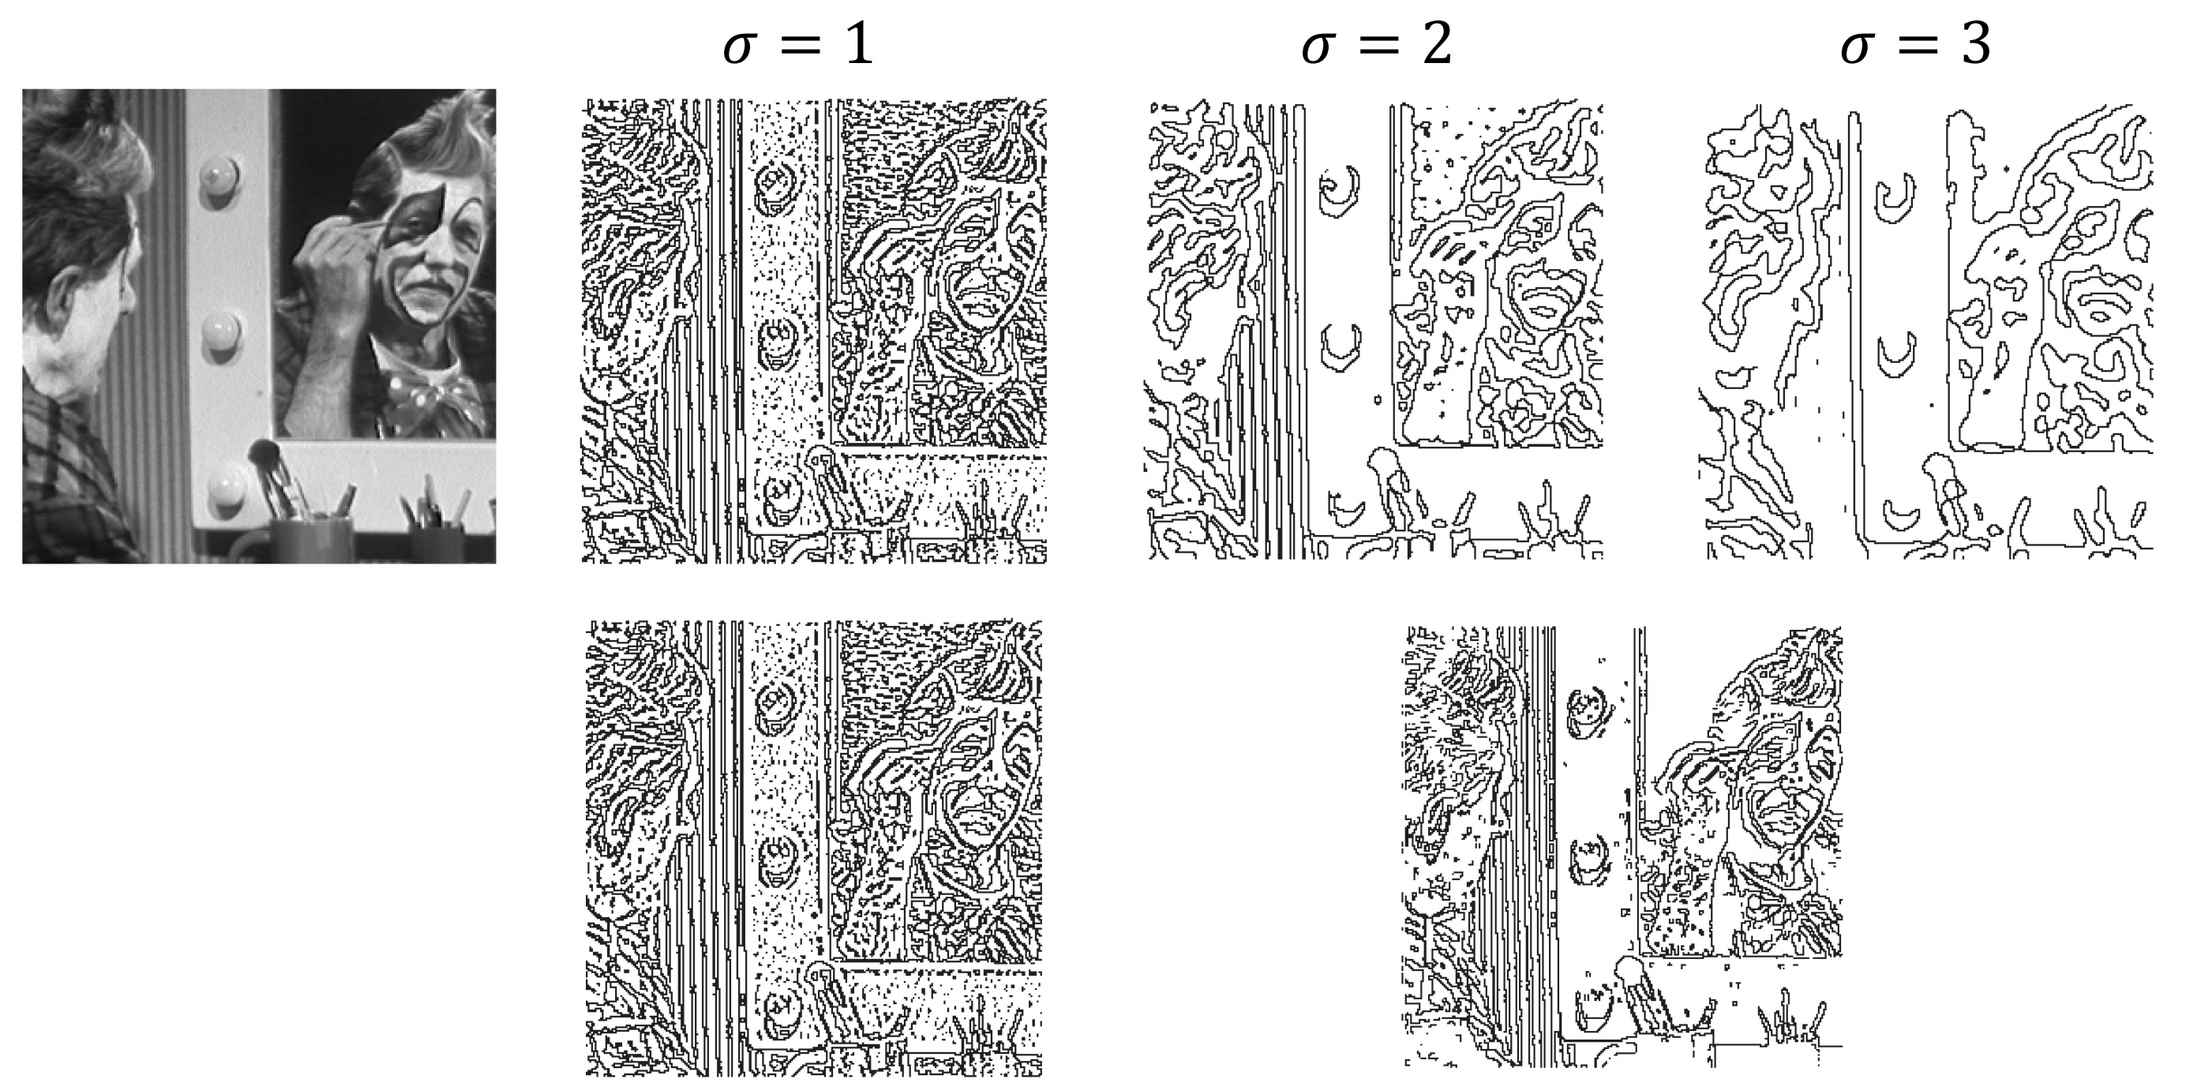
\includegraphics[width=0.7\linewidth]{./img/log_application.jpg}
  \caption{Examples of LoG application}
  \label{fig:log_application}
\end{figure}


\subsection{Feature detection and matching}
Feature detection is useful for object detection, since we can look for features in the source image and try to find them again in the target image.
Several computer vision tasks deal with finding "Corresponding Points" between two (or more) images of a scene.
Correspondences are image points which are the projection of the same 3D point in different views of the scene.
Establishing correspondences may be difficult, as the points may look different in different views.

\subsubsection{Local invariant features paradigm}
The task of establishing correspondences is split into 3 successive steps:
\begin{itemize}
  \item \textbf{Detection} of salient points.
  \item Computation of a \textbf{suitable descriptor} based on pixels in the keypoint neighbourhood.
  \item \textbf{Matching} descriptors between images.
\end{itemize}

Descriptors should be \textbf{invariant} to as many transformations as possible.
Ideally we want scale/rotation/illumination invariance.

\subsubsection{Properties of good detectors/descriptors}
\begin{itemize}
  \item Detector:
  \begin{itemize}
    \item Repeatability: it should find the same keypoints in different views of the scene despite the transformations.
    \item Saliency: it should find keypoints surrounded by informative patterns.
  \end{itemize}
  \item Descriptor:
  \begin{itemize}
    \item Distinctiveness vs. robustness trade-off: the algorithm should capture the salient information around a keypoint.
    \item Compactness: the description should be as concise as possible.
  \end{itemize}
\end{itemize}

Speed is desirable for both, and in particular for detectors, which need to be run on the whole image (while descriptors are computed at keypoints only).

Edge pixels can be hardly told apart as they look very similar along the direction perpendicular to the gradient.
Edges are locally ambiguous, since there are many other points that look just the same.

\subsubsection{Moravec Interest Point Detector}
We can define the \textbf{cornerness} at a point $p$, which is given by the minimum squared difference between the patch centered at $p$ and those centered at its 8 neighbours: 
$$C(p) = \min_{q \in n_8(p)} ||N(p) - N(q)||^2$$

\begin{figure}[htbp]
  \centering
  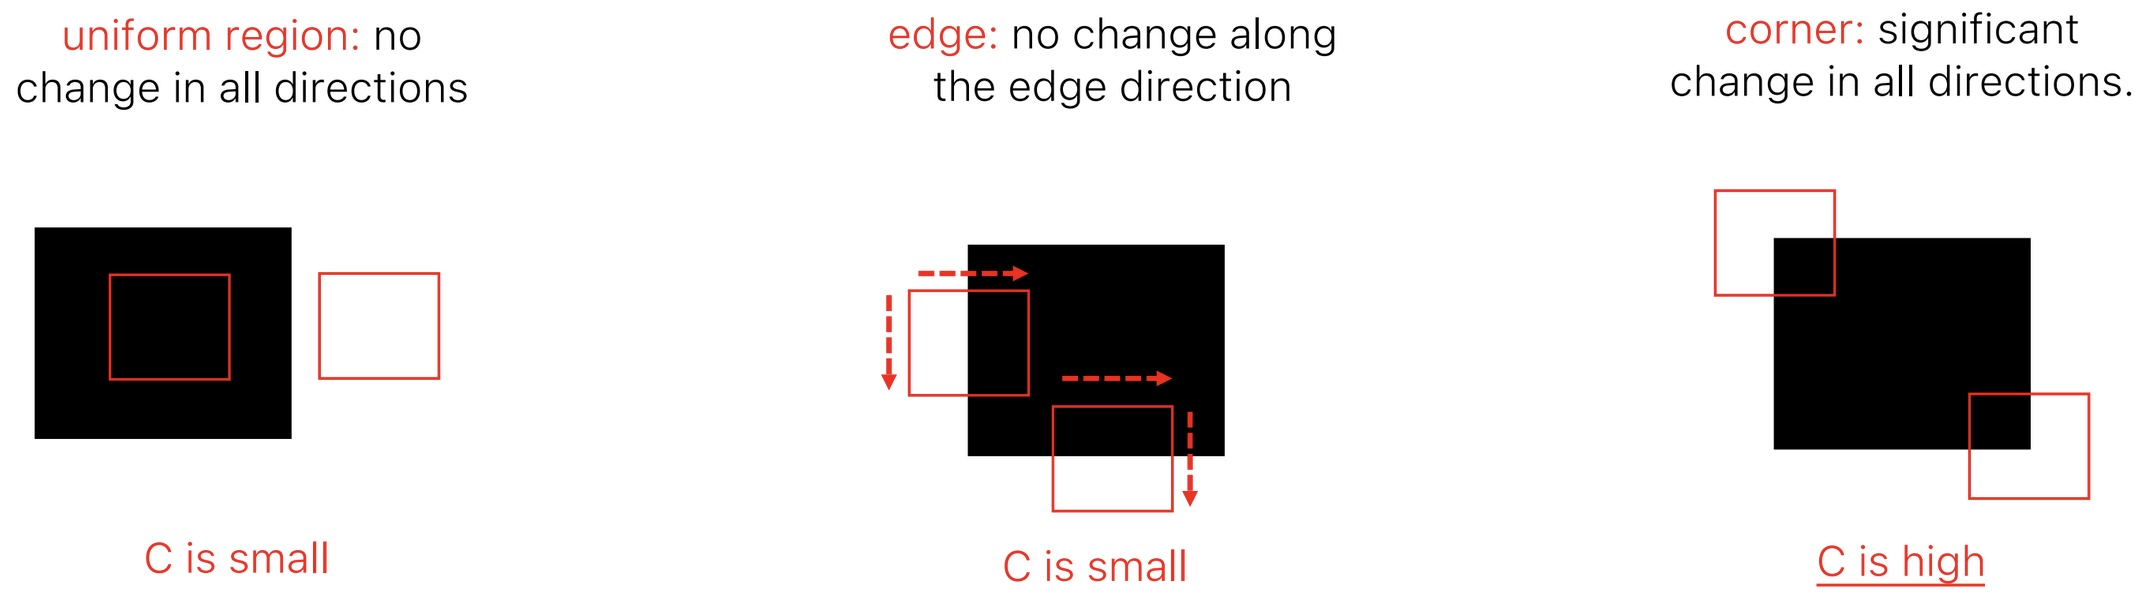
\includegraphics[width=0.9\linewidth]{./img/cornerness.jpg}
  \caption{Cornerness of an image segment}
  \label{fig:cornerness}
\end{figure}

After computing the cornerness we threshold and do Non-Maxima Suppression.

\subsubsection{Harris Corner Detector}

Harris \& Stephens proposed to rely on a continuous formulation of the Moravec's "error" function.
Assume to shift the image with a generic infinitesimal shift $(\Delta x, \Delta y)$:
$w(x,y)$ is a window set to 1 around the pixel under evaluation and 0 in all the image.
In the end we consider only the pixel around the $(x,y)$ position.

Due to the shift being infinitesimal, we can deploy Taylor's expansion of the intensity function at $(x,y)$ : $f(x + \Delta x) = f(x) + f'(x) \Delta x$

$M$ encodes the local image structure around the considered pixel.
We hypothesize that $M$ is a diagonal matrix
$M =
\begin{bmatrix}
\sum_{x,y} w(x,y) I_x(x,y)^2 & \sum_{x,y} w(x,y) I_x(x,y) I_y(x,y) \\
\sum_{x,y} w(x,y) I_y(x,y) I_x(x,y) & \sum_{x,y} w(x,y) I_y(x,y)^2
\end{bmatrix}
=
\begin{bmatrix}
\lambda_1 & 0 \\
0 & \lambda_2
\end{bmatrix}$

\begin{figure}[htbp]
  \centering
  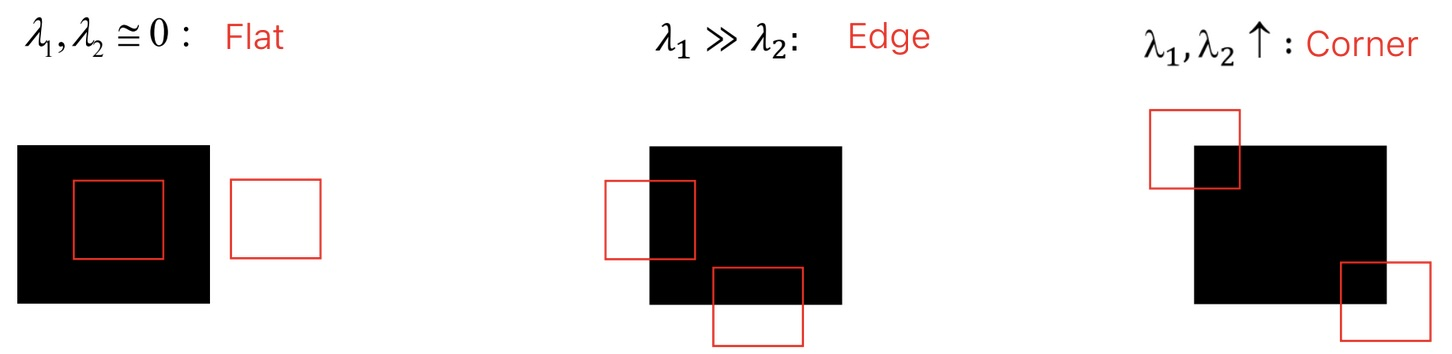
\includegraphics[width=0.9\linewidth]{./img/harris_corner_detector.jpg}
  \caption{Harris corner detector and lambda values}
  \label{fig:harris_corner_detector}
\end{figure}

The previous considerations have general validity as $M$ is real and symmatric, and thus can always be diagonalized by a rotation of the image coordinate system.
$$M = R\begin{bmatrix} \lambda_1 & 0 \\ 0 & \lambda_2 \end{bmatrix}R^T$$
The columns of $R$ are the orthogonal unit eigenvectors of $M$.
$\lambda_i$ are the corresponding eigenvalues.
$R^T$ is the rotation matrix that aligns the image axes to the eigenvectors of M.

Computing eigenvalues at each pixel is costly, so we can compute a more efficient "cornerness" function that gives a result $C$ that is positive on a corner, negative on an edge an about 0 on a flat surface.

The \textbf{Harris corner detection algorithm} can thus be summarized as follows:
\begin{enumerate}
  \item Compute $C$ at each pixel.
  \item Select all pixels where $C$ is higher than a chosen positive threshold $T$.
  \item Within the previous set, detect as corners only those pixels that are local maxima of $C$ (NMS).
\end{enumerate}

Eigenvalues of $M$ are invariant to a rotation of the image axes, and thus so is Harris cornerness function.
It also invariant to additive intensity changes.
However, it's not invariant to scale changes, as corner structures may degrade or transform into edges under significant scaling, nor to multiplicative intensity variations which scale gradients and alter the corner response magnitude unless thresholds are adaptively adjusted.

\subsubsection{Scale-Space}
Scale invariance is the main issue adressed by second generation local invariant features.
The key idea is to apply a fixed-size detection tools on increasingly down-sampled and smoothed versions of the input image.

\begin{figure}[htbp]
  \centering
  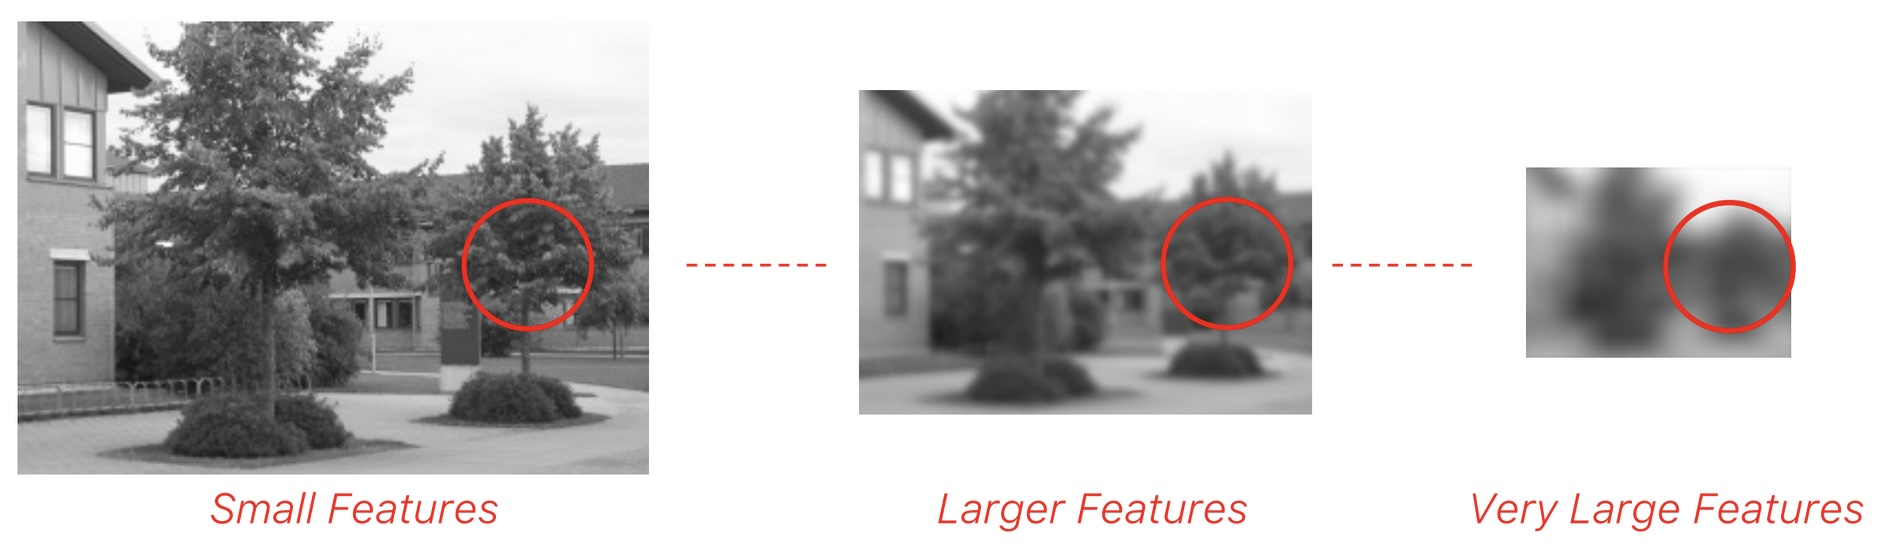
\includegraphics[width=0.9\linewidth]{./img/scale_space.jpg}
  \caption{We increase the blur as we reduce the image size}
  \label{fig:scale_space}
\end{figure}

As we move along scales, small details should continuously disappear and no structure should be introduced.

A Scale-Space is a \textbf{one-parameter family of images} created from the original one so that the structures at smaller scales are successively suppressed by smoothing operations.

A Scale-Space must be realized by Gaussian Smoothing: $L(x,y,\sigma) = G(x,y,\sigma) * I(x,y)$.
A Scale-Space is created by repeatedly smoothing the original image with larger and larger Gaussian kernels.

\paragraph{Feature Detection \& Scale Selection}
% The Gaussian Scale-Space is only a tool to represent the input image at different scales.
% It neither inclues any criterion to detect features nor to select their characteristic scale.
As features exist across a range of scales how do we establish at which scale a feature turns out maximally interesting and should therefore be described?

% The fundamental research work on multi-scale feature detection and automatic scale selection was proposed in "Feature detection with automatic scale selection" by T. Lidneberg in 1998.

As we filter more by using a higher sigma, derivatives tends to become weaker.
To compensate, Lindeberg proposed to multiply/normalize derivatives by sigma (doing scale-normalization).

\paragraph{Scale-Normalized LoG}

The scale-normalized Laplacian Of Gaussian (LoG) is: 
$$F(x,y,\sigma) = \sigma^2\nabla^2 L(x,y,\sigma) = \sigma^2(\nabla^2 G(x,y,\sigma) * I(x,y))$$ where $\sigma^2$ is the normalization factor.

The \textbf{scale-normalized LoG detects blobs} (regions with intensity variations) by combining Gaussian Smoothing (which reduces noise and suppresses fine details) and Laplacian Operator (which highlights regions of rapid intensity change).

Scale normalization is introduced since the raw LoG response diminishes as the scale ($\sigma$) increases, biasing detection toward smaller blobs.

\begin{figure}[htbp]
  \centering
  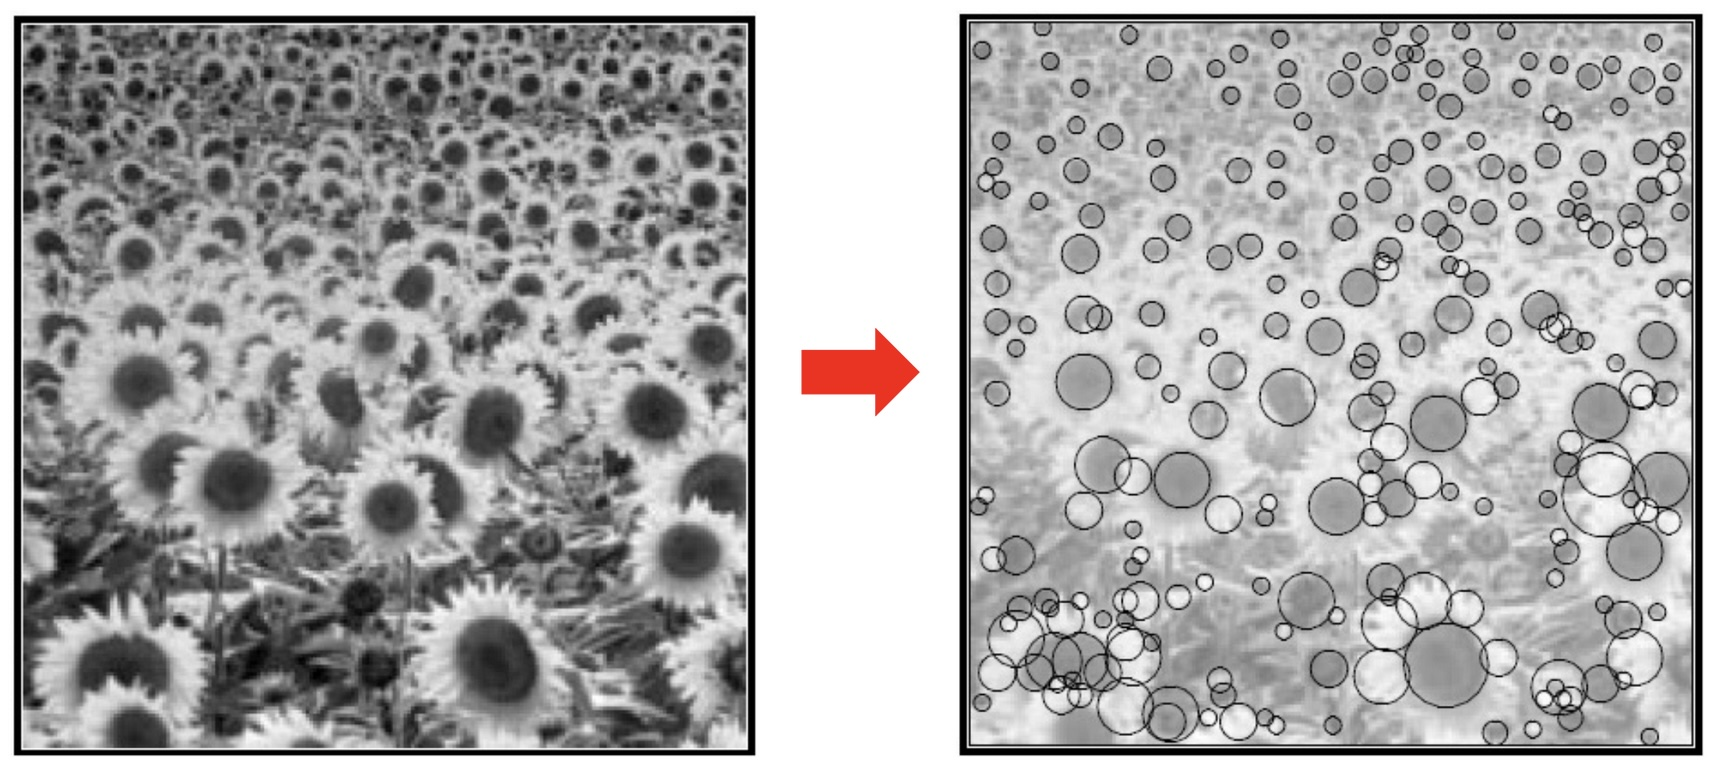
\includegraphics[width=0.7\linewidth]{./img/sunflower_blobs.jpg}
  \caption{LoG filter locates blobs}
  \label{fig:sunflower_blobs}
\end{figure}

\paragraph{Difference of Gaussian (DoG)}

Lowe proposed to detect keypoints by seeking for the extrema of the DoG (Difference of Gaussian) function across the $(x,y,\sigma)$ domain.

$$DoG(x,y,\sigma) = (G(x,y,k\sigma) - G(x,y,\sigma)) * I(x,y) = L(x,y,k\sigma) - L(x,y,\sigma)$$

This approach provides a computationally efficient approximation of Lindeberg's scale-normalized LoG.

$$G(x,y,k\sigma) - G(x,y,\sigma) \approx (k-1)\sigma^2\nabla^2 G(x,y,\sigma) * I(x,y)$$

Both detectors are rotation invariant and find blob-like features.

\begin{figure}[htbp]
  \centering
  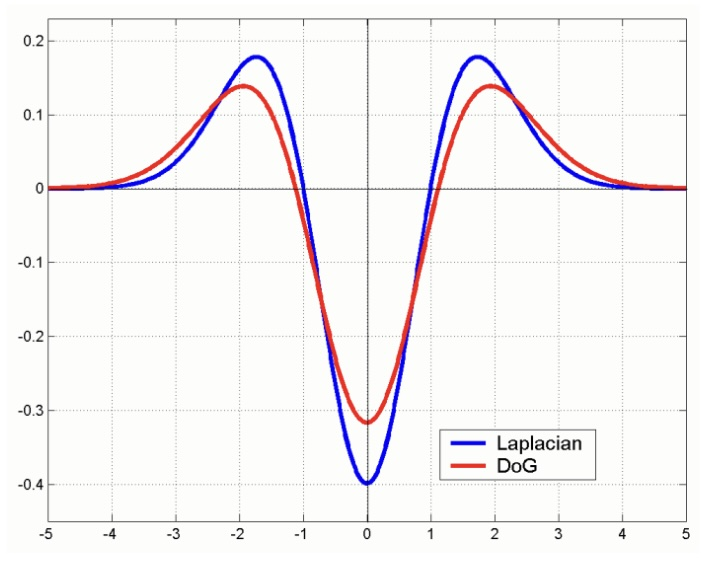
\includegraphics[width=0.5\linewidth]{./img/dog.jpg}
  \caption{Lowe proves that this is a scaled version of Lindeberg}
  \label{fig:dog}
\end{figure}

In the DoG we compute several Gaussian smoothed functions within an octave.
For each pair we take the differences, then we seek for extrema in the DoG.

\begin{figure}[htbp]
  \centering
  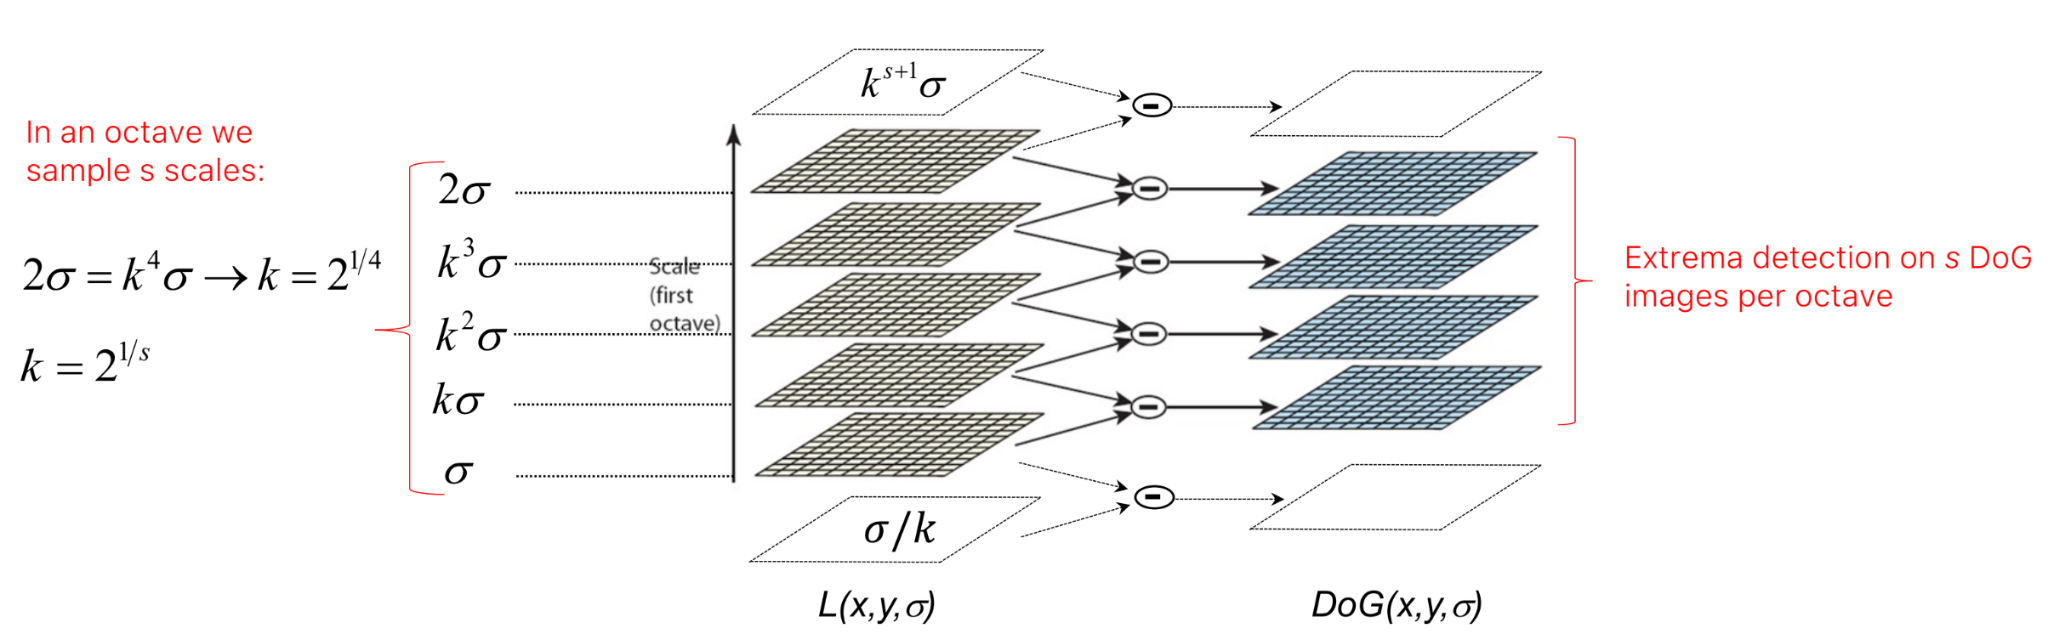
\includegraphics[width=0.9\linewidth]{./img/dog_1.png}
  \caption{Difference of Gaussian}
  \label{fig:dog_1}
\end{figure}

\paragraph{Extrema detection}
A point $(x,y,\sigma)$ is detected as a keypoint if and only if its DoG is higher (or lower) than that of the 26 neighbour (8 at the same scale and $18 =  9 + 9$ at the two nearby scales) in the $(x,y,\sigma)$ space.

According to the original article the best number of sclaes within an octave is $s=3$, initial $\sigma$ for each octave should be $\sigma =1.6$ and the input image is enlarged by a factor of 2 in both dimensions.

After detecting points as local extrema, the next step is to prune weak and unstable responses to ensure robustness.
Keypoints with low contrast, corresponding to weak DoG responses, are often sensitive to noise and less repeatable across different images.

\begin{figure}[htbp]
  \centering
  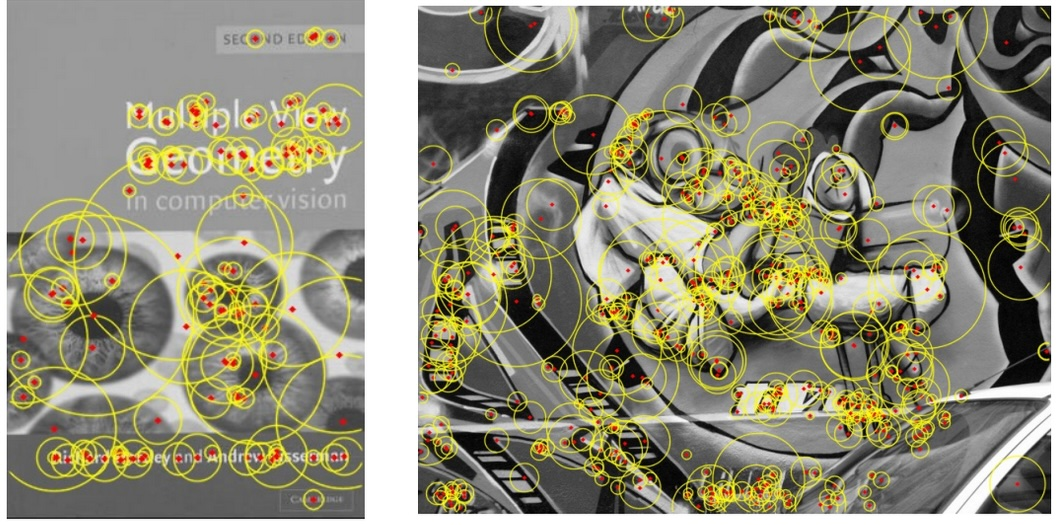
\includegraphics[width=0.7\linewidth]{./img/dog_keypoints.jpg}
  \caption{The size of the circle is proportional to the scale of the feature ($\sigma$)}
  \label{fig:dog_keypoints}
\end{figure}

\subsubsection{Scale and Rotation Invariance Description}

DoG are \textbf{rotation invariant because of circular simmetry}.
Once each keypoint has been extracted, a surrounding patch is considered to compute its descriptor (scale and rotation invariant).

We need to identify a \textbf{prominent direction} inherent to the patch (the canonical orientation) and, based on such direction, define a local reference frame.
A reasonable choice consists in identifying the \textbf{direction along which most of the gradient is found}.

To compute the canoncial orientation we need to define a scale and rotation invariant description.
Once each keypoint has been extracted, a surrounding patch is considered to compute its descriptor (scale and rotation invariant).
\begin{itemize}
  \item Scale invariance: the patch is taken from the stack of images that correspond to the characteristic scale.
  \item Rotation invariance: a canonical patch orientation is computed, so that the descriptor can then be computed on a canonically-oriented patch (orientation with respect to a new reference system, not the one of the image).
\end{itemize}

Lowe proposed to compute the \textbf{canoncial orientation of DoG keypoints} as follows: given the keypoint, the magnitude and orientation of the gradient are computed at each pixel of the associated Gaussian-smoothed image, L:

\begin{itemize}
  \item $m(x,y) = \sqrt{(L(x+1,y)-L(x-1,y))^2 + (L(x,y+1) - L(x,y-1))^2}$
  \item $\theta(x,y) = \tan^{-1}\frac{L(x,y+1)-L(x,y-1)}{L(x+1,y)-L(x-1,y)}$
\end{itemize}

We can then compute an \textbf{orientation histogram} by accumulating the contributions of the pixels belongigng to a neighborhood of the keypoint location (a bin size of $10\deg$).
The characteristic orientation of the keypoint is given by the highest peak of the orientation histogram.
Other peaks higher than $80\%$ of the main one would be kept as well.
A keypoint may have multiple canonical orientations and, in turn, multiple descriptors sharing the same location/scale with diverse orientations (this happen rarely, about on 15\% of the keypoints).

\begin{figure}[htbp]
  \centering
  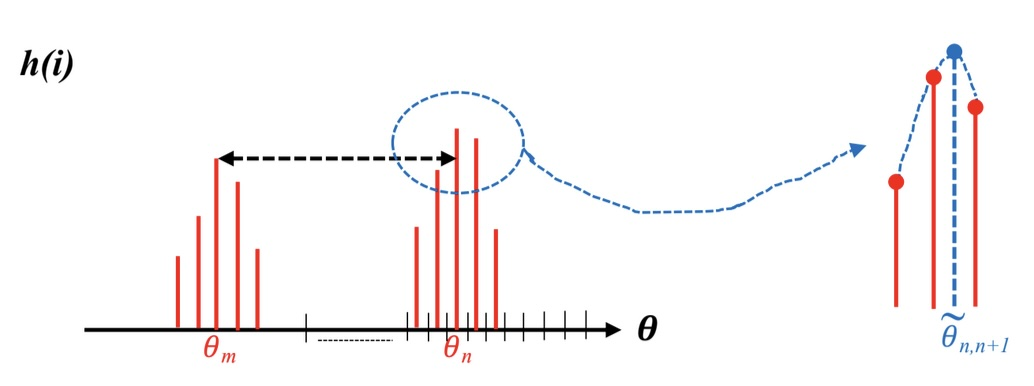
\includegraphics[width=0.7\linewidth]{./img/ambiguous_keypoint.jpg}
  \caption{This is an ambiguous keypoint, we have two prominent decisions}
  \label{fig:ambiguous_keypoints}
\end{figure}

\subsubsection{SIFT Descriptor}

The \textbf{SIFT (Scale Invariant Feature Transform)} descriptor is computed as follows:
\begin{itemize}
  \item $16\times 16$ oriented pixel grid around each keypoint is considered.
  \item This is further divided into $4 \times 4$ regions (each of size $4\times4$ pixels).
  \item A gradient orientation histogram is created for each region.
  \item Each histogram has 8 bins.
  \item Each pixel in the region contributes to its designated bin according to gradient magnitude and gaussian weighting function centered at the keypoint (with $\sigma$ equal to half the grid size).
\end{itemize}

\begin{figure}[htbp]
  \centering
  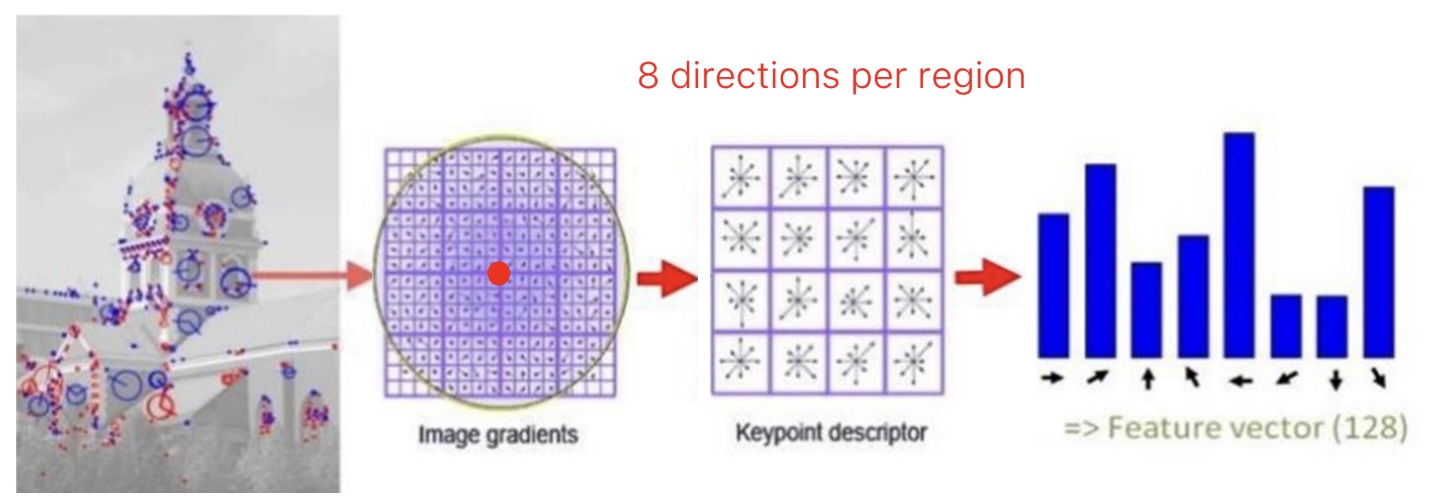
\includegraphics[width=0.8\linewidth]{./img/sift_descriptor.jpg}
  \caption{The descriptor size is given by the number of regions times the number of histogram bins per region}
  \label{fig:sift_descriptor}
\end{figure}

\paragraph{Matching process}
The descriptor is normalized to unit length to gain invariance with respect to affine intensity changes.
Descriptors like SIFT are compared across diverse views of a scene to find corresponding keypoints.
This is a classical Nearest Neighbour (NN) seach problem.
Given a set $S$ of points, $p_i$, in a matric space $M$ and a query point $q \in M$, find the $p$, closest to $q$.
We wish to match the local features computed from an image under analysis (target image $T$) to those already computed from a reference image ($R$) or a set of reference images.

For each feature in $T$ we look for the most similar one in $R$:
\begin{itemize}
  \item The features in $T$ represent the query points, $q$.
  \item The features in $R$ provide set $S$.
  \item When matching SIFT descriptors the distance typically used is the Euclidean distance.
\end{itemize}

\begin{figure}[htbp]
  \centering
  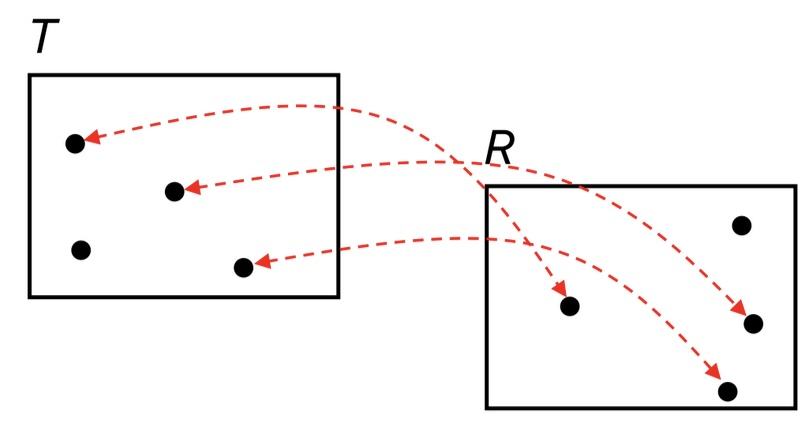
\includegraphics[width=0.5\linewidth]{./img/matching_sift.jpg}
  \caption{Image matching process with SIFT}
  \label{fig:matching_sift}
\end{figure}

The found Nearest Neighbour (NN) does not necessarily provide a valid correspondence as some features in $T$ may not have a corresponding feature in $R$.
We enforce a criteria to accept/reject a match found by the NN search process.
The simplest thing to do is to use a threshold.
Lowe showed that $T=0.8$ may allow for rejecting $90\%$ of the wrong matches while missing only $5\%$ of those correct.

Exhaustively searching for the NN of the query feature, $q$, has linear complexity in the size of $S$.
This is slow, so efficient indexing techniques are exploited to speed-up the NN-search process.
The main indexing technique exploited for feature matching is known as k-d tree.

\subsection{Camera Calibration}

Camera Calibration is important for taking quantitative measurements from images.
In the \textbf{perspective projection} model, given a point in the 3D space $M = [x,y,z]^T$, with coordinates given in the Camera Reference Frame (CRF).
Its projection onto the image plane I is denoted as $m=[u,v]^T$.

\begin{figure}[htbp]
  \centering
  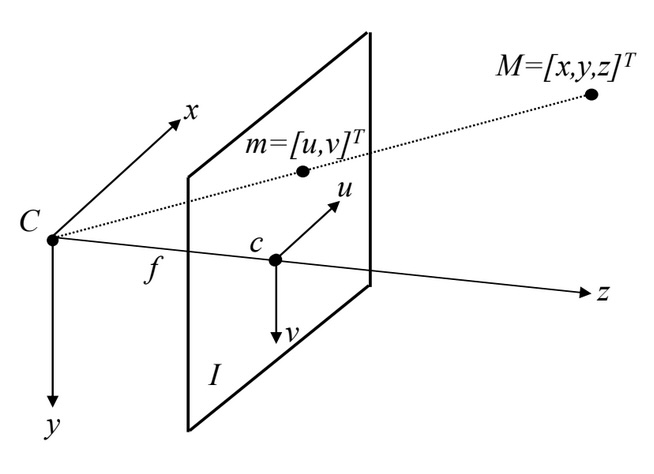
\includegraphics[width=0.5\linewidth]{./img/camera_calibration.jpg}
  \caption{Perspective Projection Model (PPM)}
  \label{fig:camera calibration}
\end{figure}

\subsubsection{Projective Space}

The \textbf{Physical Space} is a 3D Euclidean Space ($\mathbb{R}^3$) whose points can be represented as 3D vectors in a given reference frame.
In this space parallel lines do not intersect.
Points at infinity cannot be represented in this vector space.

The \textbf{Projective Space} is a mathematical engine to handle the geometry of image formations.
In the Projective space we append one more coordinate to the Euclidean triplets.
A point is represented by an equivalence class of quadruples, wherein equivalent quadruples differ just by a multiplicative factor.
This is called the \textbf{homogeneous coordinates} representation of the 3D point having Euclidean coordinates $(x,y,z)$.
The space associated with the homogeneous coordinate's representation is called Projective Space, denoted as $P^3$

\vspace{0.6em}
We are interested in Projective Spaces because Perspective Projection is \textbf{more conveniently} dealt with using projective coordinates.
\vspace{0.6em}

The point at infinity is a point in the space, the vanishing point is a point into the image plane.
Points at infinity of the 3D lines are the points of the 3D Projective Space \textbf{having the fourth coordinate equal to 0}.

To map such points into the Euclidean Space we would divide by the fourth coordinate (which is 0) which is not a valid representation in the Euclidean Space.

The point $(0,0,0,0)$ it's not the origin, but an undefined point. The origin is represented in homogeneous coordinates as $(0,0,0,k)$, with $k\neq 0$.

Given a 3D point $\tilde{M} = [x,y,z]^T$ (with coordinates expressed in the Camera Reference Frame) and its 2D projection onto the image plane $\tilde{m} = [u,v]^T$.

In homogeneous coordinates the perspective projection becomes a linear transformation.

$$
\begin{bmatrix}
u \\ v \\ 1
\end{bmatrix} =
\begin{bmatrix}
f & 0 & 0 & 0 \\
0 & f & 0 & 0 \\
0 & 0 & 1 & 0 
\end{bmatrix}
\begin{bmatrix}
x \\ y \\ z \\ 1
\end{bmatrix}
$$

Which in matrix notation is $\tilde{m} \approx \tilde{P}\tilde{M}$, where $\approx$ means "equal up to an arbitrary scale factor".
\vspace{1em}
$\tilde{P}$ represents the geometric camera model, and is known as \textbf{Perspective Projection Matrix (PPM)}.
\vspace{1em}
The operation carried out by the PPM is that of scaling lateral coordinates according to the distance from the camera $(z)$.
The actual focal length just introduces an additional scaling factor of projected coordinates.

The is just an abstraction, which is quite convenient but also useless, since there is no way to measure world coordinates in a reference frame which is basically an abstraction of a camera.

\subsubsection{A more comprehensive camera model}

To come up with a really useful camera model we need to take in account two additional issues:
\begin{itemize}
  \item Image digitization.
  \item The 6 DOF rigid motion between the Camera Reference Frame (CRF) and the World Reference Frame (WRF).
\end{itemize}

Digitization can be accounted for by including into the projection equations the scaling factors along the two axis due to the quantization associated with the horizontal and vertical pixel size, this is because we have a discrete grid of pixels.

We also need to model the translation of the piercing point (intersection between the optical axis and the image plane) with respect to the origin of the image coordinate system.
This is needed to move the reference frame from the center of the CMOS in the camera to the top left corner, since we don't want to use negative coordinates.

\subsubsection{Intrinsic Parameter Matrix}
Now the Perspective Projection Matrix can be written as:
$$
\tilde{P} = 
\begin{bmatrix}
  fk_u & 0 & u_0 & 0 \\
  0 & fk_v & v_0 & 0 \\
  0 & 0 & 1 & 0 
\end{bmatrix}
=
\begin{bmatrix}
  fk_u & 0 & u_0 \\
  0 & fk_v & v_0 \\
  0 & 0 & 1 
\end{bmatrix}
\begin{bmatrix}
  1 & 0 & 0 & 0 \\
  0 & 1 & 0 & 0 \\
  0 & 0 & 1 & 0 
\end{bmatrix}
= A[I|0]
$$

Matrix $A$, models the characteristics of the image sensing device and is called \textbf{Intrinstic Parameter Matrix}
The smallest number of intrinsic parameters is thus 4.
The intrinstic parameter matrix contains infromation about: focal length, pixel dimension and camera center.

\subsubsection{Rigid motion between CRF and WRF}
We need to apply a roto-translation to relate the World Reference Frame to the Camera Reference Frame.
The relation between the coordinates of a point in the two reference frames is:

$$
W =
\begin{bmatrix}
X \\ Y \\ Z \\ 1
\end{bmatrix}
\,,
M=
\begin{bmatrix}
x\\ y\\ z\\1
\end{bmatrix}
\Rightarrow
M=
\begin{bmatrix}
R & T \\
0 & 1
\end{bmatrix}
W = GW
$$

% TODO: REVISE AFTER NEW LESSON DROP
To map a 3D point expressed in the Camera Reference Frame: $k\tilde{m} = A[I|0]\tilde{M}$

The general from of the Perspective Projection Matrix can be expressed as follows:
$\tilde{P} = A[I|0]G$ or also $\tilde{P}=A[R|T]$.

\paragraph{Extrinsic Parameters}

$G$ is called \textbf{Extrinsic Parameter Matrix} and it encodes the position and orientation of the camera with respect to the World Reference Frame.
The rotation matrix has only 3 independent parameters, which correspond to the rotation angles around the axis of the reference frame.
$T$ has 3 independent parameters.
The total number of \textbf{extrinsic parameters} is 6 (3 translation, 3 rotation).
$A$ has 4 independent parameters.
The general form of the Perspective Projection Matrix can be thought of as encoding:
\begin{itemize}
  \item the position of the camera with respect to the world into $G$.
  \item the actual characteristics of the sensing device into $A$.
\end{itemize}

\subsubsection{P as a Homography}
We just need the relation between the camera and the plane, then we can measure everything on that plane.

If the camera is imaging a planar scene, we can assume the z-axis of the World Reference Frame to be perpendicular to the plane such that all 3D points will have their z-coordinate equal to 0.
The Perspective Projection Matrix then becomes a simpler transformation defined by a $3x3$ matrix.
$$k\tilde{m} = \tilde{P}\tilde{w}
\begin{bmatrix}
  p_{1,1} & p_{1,2} & \cancel{p_{1,3}} & p_{1,4} \\
  p_{2,1} & p_{2,2} & \cancel{p_{2,3}} & p_{2,4} \\
  p_{3,1} & p_{3,2} & \cancel{p_{3,3}} & p_{3,4} 
\end{bmatrix}
\begin{bmatrix}
x \\ y \\ 0 \\ 1
\end{bmatrix}
=
\begin{bmatrix}
  p_{1,1} & p_{1,2} & p_{1,4} \\
  p_{2,1} & p_{2,2} & p_{2,4} \\
  p_{3,1} & p_{3,2} & p_{3,4} 
\end{bmatrix}
\begin{bmatrix}
x \\ y \\ 1
\end{bmatrix}
= H\tilde{M}
$$

Such a transformation, denoted here as H, is known as \textbf{homography} and represents a general linear transformation between projective planes.
A homography is then a projective transformation between two planes or a mapping between two planar projection of an image.

\begin{figure}[htbp]
  \centering
  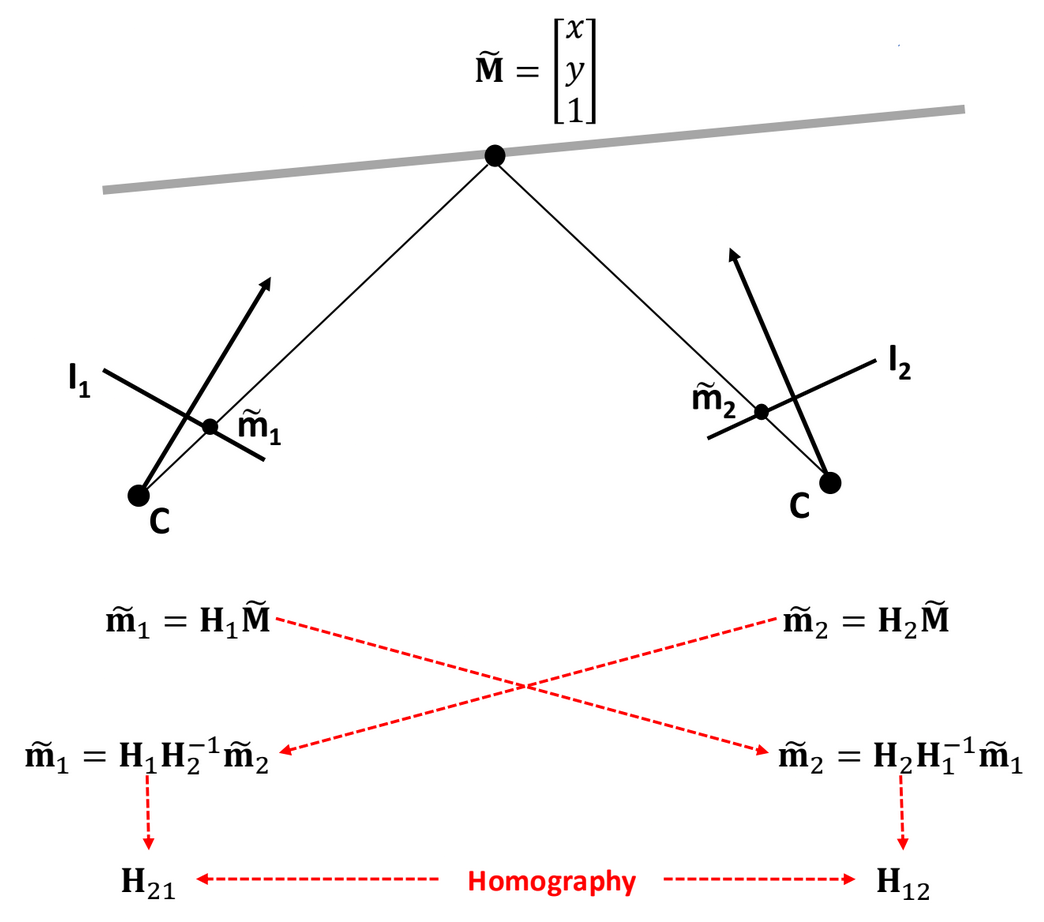
\includegraphics[width=0.6\linewidth]{./img/homography.jpg}
  \caption{Any two images of a planar scene are related by a homography}
  \label{fig:homography}
\end{figure}


\begin{figure}[htbp]
  \centering
  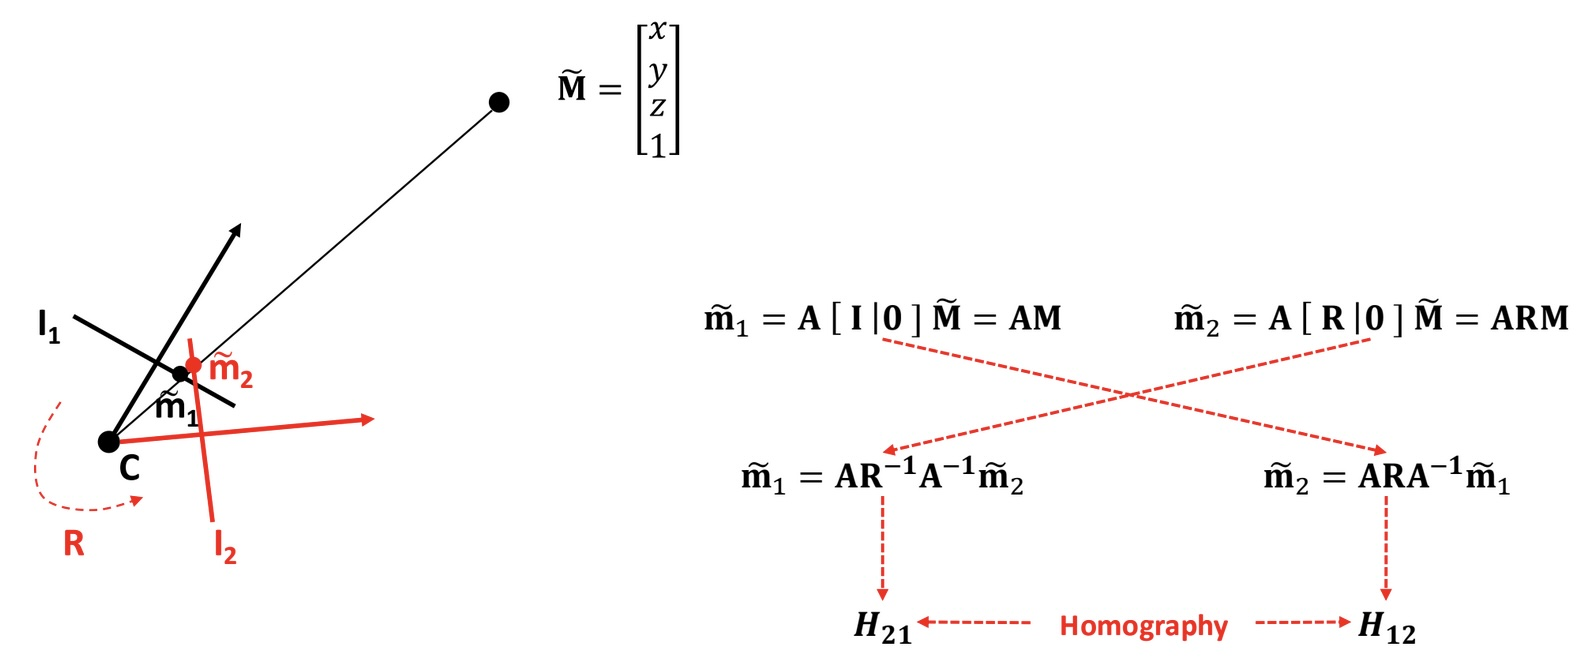
\includegraphics[width=0.8\linewidth]{./img/rotating_homography.jpg}
  \caption{Any two images taken by a camera rotating about the optical center are related by a homography}
  \label{fig:rotating_homography}
\end{figure}

\begin{figure}[htbp]
  \centering
  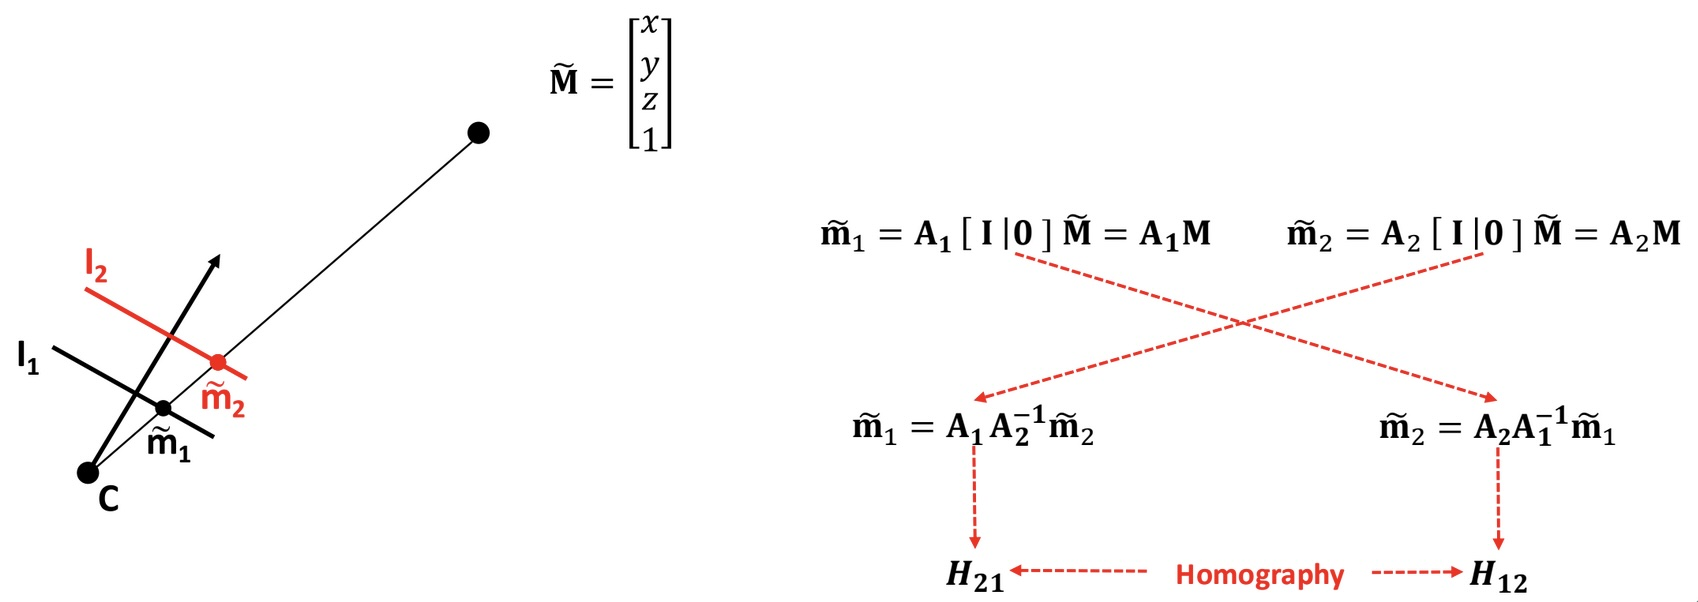
\includegraphics[width=0.8\linewidth]{./img/moving_homography.jpg}
  \caption{Any two images taken by different cameras in fexed pose are related bu a homography}
  \label{fig:moving_homography}
\end{figure}

\subsubsection{Lens distortion}

The Perspective Projection Matrix is based on the pinhole camera model, however, real lenses introduce distortions with respect to the pure pinhole model.
We also have lens distortion, which is modelled through additional parameters that don't alter the form of the Perspective Projection Matrix.

We have two types of lens distortion: barrel distortion which bends straight lines outwards, and pincushion distortion, which causes straight lines to curve inward.

\subsubsection{Calibration}

We now have the Perspective Projection Matrix camera model, which can be decomposed in:
\begin{itemize}
  \item Intrinsic parameter matrix $A$.
  \item Rotation matrix $R$.
  \item Translation vector $T$.
\end{itemize}

\textbf{Camera calibration} is the process whereby \textbf{all parameters defining the camera model are estimated} for a specific camera device.
Depending on the application, \textbf{either the Perspective Projection Matrix (PMM) only, or also its independent components} ($A$,$R$,$T$) need to be estimated.

There are many camera calibration algorithms, but the basic process always relies on setting up a linear system of equations given a set of known 3D-2D correspondences.
To obtain the correspondences we use calibration targets, which have easily detectable features.

The approaches can be split into:
\begin{itemize}
  \item Those relying on a single image containing a known pattern.
  \item Those relying on several different images of one given planar pattern.
\end{itemize}

\subsubsection{Zhang's method for Camera Calibration}

We use a chessboard pattern of which we know the number of internal corners and the size of the squares.
Internal corners can be easily detected by standard algorithms, like the Harris corner detector.
Typically the camera is fixed and you move the calibration target in front of the camera.
The $[R\,T]$ are estimated with respect to the reference system attached to the target, but it changes alongside with the pattern.
In each image the 3D world reference frame is taken at the top-left corner of the pattern.
Each image requires its own estimate of the extrinstic parameters, as they are different from one to the other.
Due to the choice of the world reference frame associated with calibration images, in each of them we consider only 3D points with $z=0$.
The Perspective Projection Matrix boils down to a simpler transformation defined by an homography $3\times 3$ matrix, like with $P$ as a homography.

$$k\tilde{m} = \tilde{P}\tilde{w}
\begin{bmatrix}
  p_{1,1} & p_{1,2} & \cancel{p_{1,3}} & p_{1,4} \\
  p_{2,1} & p_{2,2} & \cancel{p_{2,3}} & p_{2,4} \\
  p_{3,1} & p_{3,2} & \cancel{p_{3,3}} & p_{3,4} 
\end{bmatrix}
\begin{bmatrix}
x \\ y \\ \cancel{0} \\ 1
\end{bmatrix}
=
\begin{bmatrix}
  p_{1,1} & p_{1,2} & p_{1,4} \\
  p_{2,1} & p_{2,2} & p_{2,4} \\
  p_{3,1} & p_{3,2} & p_{3,4} 
\end{bmatrix}
\begin{bmatrix}
x \\ y \\ 1
\end{bmatrix}
= H\tilde{M}
$$

Given a pattern with $m$ corners, we can write $m$ systems of 3 linear equations, where:
\begin{itemize}
  \item Both 3D as well as 2D coordinates are known due to the corners having been detected in the i-th image and the unknowns are thus the 9 elements in $H_i$.
  \item $H_i$ (and $P_i$ alike) is known up to an arbitrary scale factor, the independent elements in $H_i$ are 8.
\end{itemize}

\textbf{There are plenty of methods for the estimation}

The Zhang's method can be summarized as:
\begin{enumerate}
  \item Acquire $n$ images of a planar pattern with $m$ internal corners.
  \item For each image compute an initial guess for homography $H_i$.
  \item Refine eaech $H_i$ by minimizing the reprojection error.
  \item Get an initial guess for $A$ given the homographies $H_i$.
  \item Given $A$ and $H_i$, get an initial guess for $R_i$ and $T_i$.
  \item Compute an initial guess for lens distortion parameters $k$.
  \item Refine all parameters $A$, $R_i$, $T_i$, $k$ by minimizing the reprojection error.
\end{enumerate}

\subsubsection{Image warping}

% TODO: WRITE AFTER LESSON DROP (SLIDE 38/65)

After applying the warping function you get real coordinates not discrete ones.
During the mapping, some pixels of the destination image may be not rounded perfectly.
What if more pixels go to the same position?
\begin{figure}[htbp]
  \centering
  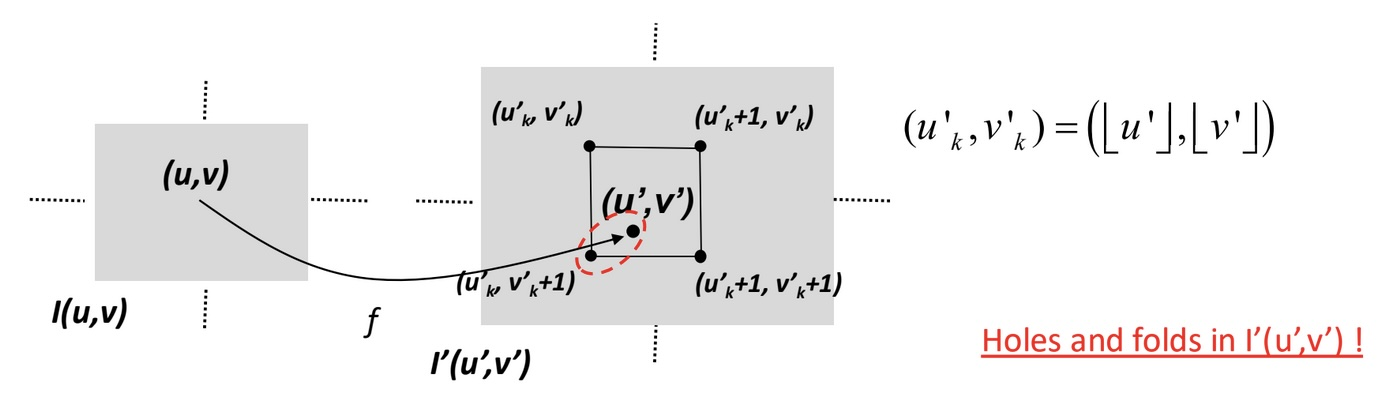
\includegraphics[width=0.8\linewidth]{./img/forward_mapping.jpg}
  \caption{A better choice consists in mapping to the closest point into the destination image}
  \label{fig:forward_mapping}
\end{figure}

Since the coordinates are always real values the different mapping strategies can be to map the closest point or to interpolate between the 4 closest points.







\vspace{3em}
\section{Advanced Topics in Deep Learning for Computer Vision}

\end{document}
